\documentclass[twoside]{article}

\usepackage{aistats2025}
\usepackage{amsmath,amssymb,amsthm}
\usepackage{graphicx}
\usepackage{subcaption}
\usepackage{xcolor}
% \usepackage{biblatex}
\usepackage{natbib}
\newcommand{\E}{\mathbb{E}}
\newcommand{\he}{\mathrm{he}}
\newcommand{\He}{\mathrm{He}}
\newtheorem{theorem}{Theorem}
\newtheorem{lemma}{Lemma}
\newtheorem{remark}{Remark}
\newtheorem{corollary}{Corollary}
\newtheorem{proposition}{Proposition}
\theoremstyle{definition}
\newtheorem{definition}{Definition}
% \newtheorem{corollary}[theorem]{Corollary}
% \let\cite\citep
% Full citations
\makeatletter
\newcommand{\upmax}{\def\blx@maxcitenames{99}}
\newcommand{\dnmax}{\def\blx@maxcitenames{1}}
\makeatother
\newcommand{\myfullcite}[1]{\upmax\fullcite{#1}\dnmax}

\newcommand\blfootnote[1]{%
  \begingroup
  \renewcommand\thefootnote{}\footnote{#1}%
  \addtocounter{footnote}{-1}%
  \endgroup
}

\newcommand{\bigo}{\mathcal{O}}



% Mark sections of captions for referring to divisions of figures
% \newcommand{\figleft}{{\em (Left)}}
% \newcommand{\figcenter}{{\em (Center)}}
% \newcommand{\figright}{{\em (Right)}}
% \newcommand{\figtop}{{\em (Top)}}
% \newcommand{\figbottom}{{\em (Bottom)}}
% \newcommand{\captiona}{{\em (a)}}
% \newcommand{\captionb}{{\em (b)}}
% \newcommand{\captionc}{{\em (c)}}
% \newcommand{\captiond}{{\em (d)}}


% Highlight a newly defined term
% \newcommand{\newterm}[1]{{\bf #1}}
% Figure reference, lower-case.
\def\figref#1{figure~\ref{#1}}
% Figure reference, capital. For start of sentence
\def\Figref#1{Figure~\ref{#1}}
\def\twofigref#1#2{figures \ref{#1} and \ref{#2}}
\def\quadfigref#1#2#3#4{figures \ref{#1}, \ref{#2}, \ref{#3} and \ref{#4}}
% Section reference, lower-case.
\def\secref#1{section~\ref{#1}}
% Section reference, capital.
\def\Secref#1{Section~\ref{#1}}
% Reference to two sections.
\def\twosecrefs#1#2{sections \ref{#1} and \ref{#2}}
% Reference to three sections.
\def\secrefs#1#2#3{sections \ref{#1}, \ref{#2} and \ref{#3}}
% Reference to an equation, lower-case.
\def\eqref#1{equation~\ref{#1}}
% Reference to an equation, upper case
\def\Eqref#1{Equation~\ref{#1}}
% A raw reference to an equation---avoid using if possible
\def\plaineqref#1{\ref{#1}}
% Reference to a chapter, lower-case.
\def\chapref#1{chapter~\ref{#1}}
% Reference to an equation, upper case.
\def\Chapref#1{Chapter~\ref{#1}}
% Reference to a range of chapters
\def\rangechapref#1#2{chapters\ref{#1}--\ref{#2}}
% Reference to an algorithm, lower-case.
\def\algref#1{algorithm~\ref{#1}}
% Reference to an algorithm, upper case.
\def\Algref#1{Algorithm~\ref{#1}}
\def\twoalgref#1#2{algorithms \ref{#1} and \ref{#2}}
\def\Twoalgref#1#2{Algorithms \ref{#1} and \ref{#2}}
% Reference to a part, lower case
\def\partref#1{part~\ref{#1}}
% Reference to a part, upper case
\def\Partref#1{Part~\ref{#1}}
\def\twopartref#1#2{parts \ref{#1} and \ref{#2}}

\def\ceil#1{\lceil #1 \rceil}
\def\floor#1{\lfloor #1 \rfloor}
\def\1{\bm{1}}

\newcommand{\IG}{\phi}
%\newcommand{\OG}{\psi}
\newcommand{\EV}{\sigma_\lambda}
\newcommand{\Loss}{\mathcal{L}}

\newcommand{\BN}{\text{\sc{Bn}}}
\newcommand{\LN}{\text{\sc{Ln}}}

% \newcommand{\diag}{\text{diag}}
\newcommand{\I}{\mathcal{I}}
\renewcommand{\det}{\text{det}}
% \newcommand{\tr}{\text{Tr}}
\newcommand{\wg}{\text{Wg}}
% \newcommand{\norm}[1]{\left\|#1\right\|}


% Iso 

\newcommand{\Cos}[2]{\rho(#1,#2)}
\newcommand{\Iso}{\mathcal{I}}
% \renewcommand{\Bar}[1]{\overline{#1}}
% \renewcommand{\Hat}[1]{\widehat{#1}}
\newcommand{\ID}{-\log\Iso}
% \newcommand{\bn}{\textsc{BN}} % Please do not remove commands
\newcommand{\Norm}[1]{\widetilde{#1}}
% \newcommand{\loss}{\ell}
\newcommand{\He}{\,\mathrm{He}}
\newcommand{\he}{\,\mathrm{he}}
% \newcommand{\1}{\mathbf{1}}
% \newcommand{\0}{\mathbf{0}}
% \newcommand{\ndet}{\mathrm{\tilde{det}}}
% \newcommand{\veps}{\varepsilon}



% \newcommand{\mean}[1]{\mu_{#1}}
% \newcommand{\Mean}[2]{M_{#1}(#2)}
% \newcommand{\var}[1]{{\sigma}_{#1}^2}
% \newcommand{\gm}{\text{G.M. }}
% \newcommand{\am}{\text{A.M. }}
% \newcommand{\iid}{{i.i.d. }}
% \newcommand{\BN}{{BN}}
% \newcommand{\LN}{{LN}}
% \newcommand{\RN}[1]{\widetilde{#1}}
% \newcommand{\CN}[1]{\widehat{#1}}
% \newcommand{\eps}{{\varepsilon}}
% \newcommand{\N}{\mathbb{N}}
% \newcommand{\R}{\mathbb{R}}
% \def\1{\bm{1}}
% \def\0{\bm{0}}
% \newcommand{\nfrac}{\nicefrac} % nice frac short-hand

% \newcommand{\adj}{\mathrm{adj}}
% \newcommand{\indic}{\mathds{1}}
% \DeclareMathOperator{\Tr}{tr}
% \newcommand{\tr}{\mathrm{tr}}
% \newcommand{\row}{{\mathrm{row}}}
% \newcommand{\col}{{\mathrm{col}}}
% \newcommand{\ip}[2]{\langle #1,#2\rangle}
% \newcommand{\diag}{\mathrm{diag}}


% \newcommand{\Comment}{\triangleright}

% \newcommand{\disteq}{\stackrel{\gD}{=}}
% \newcommand{\Expec}[1]{\operatorname{\E}\left[{#1}\right]}
% \newcommand{\Prob}[1]{\operatorname{\P}\left\{{#1}\right\}}
% \newcommand{\E}{\mathbb{E}}
% \renewcommand{\P}{\mathbb{P}}
% \newcommand{\KL}{D_{\mathrm{KL}}}
% \newcommand{\Cov}[1]{C_{#1}}
% \newcommand{\Gram}[1]{C_{#1}}
% \DeclareMathOperator*{\Var}{Var}
% \newcommand{\tv}[2]{\norm{\mu_{#1}-\mu_{#2}}_{tv}}
% \newcommand{\TV}{{{tv}}}
% \newcommand{\Unif}{\mathrm{Unif}}
% \newcommand{\Normal}{\mathcal{N}}


\newcommand{\act}{\phi}
% \newcommand{\relu}{{\mathrm{relu}}}
% \newcommand{\softmax}{\mathrm{softmax}}
% \newcommand{\sigmoid}{\sigma}
% \DeclareMathOperator{\sign}{sign}
% \newcommand{\sgn}{\mathrm{sgn}}

% \def\ceil#1{\lceil #1 \rceil}
% \def\floor#1{\lfloor #1 \rfloor}

% \DeclareMathOperator*{\argmax}{arg\,max}
% \DeclareMathOperator*{\argmin}{arg\,min}
% \let\norm\relax
% \DeclarePairedDelimiter\norm{\|}{\|}
% \newcommand{\normlzero}{L^0}
% \newcommand{\normlone}{L^1}
% \newcommand{\normltwo}{L^2}
% \newcommand{\normlp}{L^p}
% \newcommand{\lp}[2]{\norm{#1}_{{#2}}}
% \newcommand{\lone}[1]{\lp{#1}{1}}
% \newcommand{\ltwo}[1]{\lp{#1}{2}}
% \newcommand{\normmax}{L^\infty}


%%%%% NEW MATH DEFINITIONS %%%%%


% \usepackage{commath,dsfont,cleveref,nicefrac,tikz,mathtools}
% \usepackage{booktabs}

% \newtheorem{proof}{Proof}

\newtheorem{theorem}{Theorem}[theorem]
\newtheorem{lemma}[theorem]{Lemma}
\newtheorem{proposition}[theorem]{Proposition}
\newtheorem{corollary}[theorem]{Corollary}

\theoremstyle{definition}
\newtheorem{definition}[theorem]{Definition}
\newtheorem{example}[theorem]{Example}
\newtheorem{assumption}[theorem]{Assumption}
\newtheorem*{assumption*}{\assumptionnumber}


\theoremstyle{remark}
\newtheorem{remark}[theorem]{Remark}



% \newcommand{\nfrac}{\nicefrac}
\newcommand{\iid}{{i.i.d. }}
\newcommand{\eps}{{\varepsilon}}
\newcommand{\C}{{G_*}}
\newcommand{\Csa}{G}
\renewcommand{\O}{{O}}
\newcommand{\A}{A_{\infty}}
\newcommand{\Hbar}{\overline{\H}}
\newcommand{\OPT}{\lambda_1^{-1}}

\newcommand{\indic}{\mathds{1}}
\newcommand{\TV}{{{tv}}}
\newcommand{\Bern}{\mathrm{Bern}}
\newcommand{\adj}{\mathrm{adj}}
\def\ones{{\bm{1}}}
\newcommand{\sr}{\text{sr}}

\newcommand{\Comment}{\triangleright}
\newcommand{\nhalf}{{\nicefrac{-1}{2}}}
\newcommand{\half}{{\nicefrac{1}{2}}}
\newcommand{\E}{\mathbb{E}}
\renewcommand{\P}{\mathbb{P}}
\newcommand{\nfrac}{\nicefrac} % nice frac short-hand
\newcommand{\Expec}[1]{\operatorname{\E}\left[{#1}\right]}
\newcommand{\Prob}[1]{\operatorname{\P}\big\{{#1}\big\}}
\newcommand{\N}{\mathbb{N}}
\newcommand{\R}{\mathbb{R}}
\newcommand{\eqdist}{\stackrel{\mathcal{D}}{\equiv} }
\def\1{\bm{1}}
\def\0{\bm{0}}
\let\norm\relax
% \DeclarePairedDelimiter\norm{\|}{\|}
\renewcommand{\r}[1]{\bm{#1}}

\newcommand{\row}{{\mathrm{row}}}
\newcommand{\couple}{{\delta}}
\newcommand{\F}{{\sigma}}
\newcommand{\G}{{G}}
\newcommand{\M}{\mathbb{M}}
\newcommand{\distort}{{B}}
\newcommand{\relu}{{\mathrm{relu}}}
% \newcommand{\normop}{\phi}
% \newcommand{\bn}{{\normop}_{p}}
% \newcommand{\BN}{{\phi}}
% \newcommand{\bn}{\normop_{\text{proj.}}}
% \newcommand{\BN}{\normop_{\text{std.}}}
\newcommand\myfrac[2]{\frac{#1\mathstrut}{#2}}    

% \DeclareSymbolFont{largesymbols}{OMX}{cmex}{m}{n}


\newcommand{\T}{\mathcal{T}}
\newcommand{\sgn}{\mathrm{sgn}}
\newcommand{\ip}[2]{\langle #1,#2\rangle}
\newcommand{\Unif}{\mathrm{Unif}}
\newcommand{\Normal}{\mathcal{N}}
\newcommand{\diag}{\mathrm{diag}}
\newcommand{\Cov}{\mathrm{Cov}}
\newcommand{\tr}{\mathrm{tr}}
\DeclareMathOperator*{\argmax}{arg\,max}
\DeclareMathOperator*{\argmin}{arg\,min}
\DeclareMathOperator*{\Var}{Var}

\newcommand{\ChainUpdate}{\mathcal{T}}
\newcommand{\Fsub}{\gF_{\text{sub-lin}}}
\newcommand{\Fgain}{\gF_{\text{gain-}\beta}}
\newcommand{\Fodd}{\gF_{\text{odd}}}
\renewcommand{\H}{\mathcal{H}}
\newcommand{\MI}{\mathcal{I}}
\newcommand{\MInorm}{\overline{\MI}}
\newcommand{\fodd}{\mathcal{F}_{\text{odd}}}
\newcommand{\tv}[2]{\norm{\mu_{#1}-\mu_{#2}}_{tv}}




% Mark sections of captions for referring to divisions of figures
\newcommand{\figleft}{{\em (Left)}}
\newcommand{\figcenter}{{\em (Center)}}
\newcommand{\figright}{{\em (Right)}}
\newcommand{\figtop}{{\em (Top)}}
\newcommand{\figbottom}{{\em (Bottom)}}
\newcommand{\captiona}{{\em (a)}}
\newcommand{\captionb}{{\em (b)}}
\newcommand{\captionc}{{\em (c)}}
\newcommand{\captiond}{{\em (d)}}

% Highlight a newly defined term
\newcommand{\newterm}[1]{{\bf #1}}


% Figure reference, lower-case.
\def\figref#1{figure~\ref{#1}}
% Figure reference, capital. For start of sentence
\def\Figref#1{Figure~\ref{#1}}
\def\twofigref#1#2{figures \ref{#1} and \ref{#2}}
\def\quadfigref#1#2#3#4{figures \ref{#1}, \ref{#2}, \ref{#3} and \ref{#4}}
% Section reference, lower-case.
\def\secref#1{section~\ref{#1}}
% Section reference, capital.
\def\Secref#1{Section~\ref{#1}}
% Reference to two sections.
\def\twosecrefs#1#2{sections \ref{#1} and \ref{#2}}
% Reference to three sections.
\def\secrefs#1#2#3{sections \ref{#1}, \ref{#2} and \ref{#3}}
% Reference to an equation, lower-case.
\def\eqref#1{equation~\ref{#1}}
% Reference to an equation, upper case
\def\Eqref#1{Equation~\ref{#1}}
% A raw reference to an equation---avoid using if possible
\def\plaineqref#1{\ref{#1}}
% Reference to a chapter, lower-case.
\def\chapref#1{chapter~\ref{#1}}
% Reference to an equation, upper case.
\def\Chapref#1{Chapter~\ref{#1}}
% Reference to a range of chapters
\def\rangechapref#1#2{chapters\ref{#1}--\ref{#2}}
% Reference to an algorithm, lower-case.
\def\algref#1{algorithm~\ref{#1}}
% Reference to an algorithm, upper case.
\def\Algref#1{Algorithm~\ref{#1}}
\def\twoalgref#1#2{algorithms \ref{#1} and \ref{#2}}
\def\Twoalgref#1#2{Algorithms \ref{#1} and \ref{#2}}
% Reference to a part, lower case
\def\partref#1{part~\ref{#1}}
% Reference to a part, upper case
\def\Partref#1{Part~\ref{#1}}
\def\twopartref#1#2{parts \ref{#1} and \ref{#2}}

\def\ceil#1{\lceil #1 \rceil}
\def\floor#1{\lfloor #1 \rfloor}
\newcommand{\train}{\mathcal{D}}
\newcommand{\valid}{\mathcal{D_{\mathrm{valid}}}}
\newcommand{\test}{\mathcal{D_{\mathrm{test}}}}


% Random variables
\def\reta{{\textnormal{$\eta$}}}
\def\ra{{\textnormal{a}}}
\def\rb{{\textnormal{b}}}
\def\rc{{\textnormal{c}}}
\def\rd{{\textnormal{d}}}
\def\re{{\textnormal{e}}}
\def\rf{{\textnormal{f}}}
\def\rg{{\textnormal{g}}}
\def\rh{{\textnormal{h}}}
\def\ri{{\textnormal{i}}}
\def\rj{{\textnormal{j}}}
\def\rk{{\textnormal{k}}}
\def\rl{{\textnormal{l}}}
% rm is already a command, just don't name any random variables m
\def\rn{{\textnormal{n}}}
\def\ro{{\textnormal{o}}}
\def\rp{{\textnormal{p}}}
\def\rq{{\textnormal{q}}}
\def\rr{{\textnormal{r}}}
\def\rs{{\textnormal{s}}}
\def\rt{{\textnormal{t}}}
\def\ru{{\textnormal{u}}}
\def\rv{{\textnormal{v}}}
\def\rw{{\textnormal{w}}}
\def\rx{{\textnormal{x}}}
\def\ry{{\textnormal{y}}}
\def\rz{{\textnormal{z}}}

% Random vectors
\def\rvepsilon{{\mathbf{\epsilon}}}
\def\rvtheta{{\mathbf{\theta}}}
\def\rva{{\mathbf{a}}}
\def\rvb{{\mathbf{b}}}
\def\rvc{{\mathbf{c}}}
\def\rvd{{\mathbf{d}}}
\def\rve{{\mathbf{e}}}
\def\rvf{{\mathbf{f}}}
\def\rvg{{\mathbf{g}}}
\def\rvh{{\mathbf{h}}}
\def\rvu{{\mathbf{i}}}
\def\rvj{{\mathbf{j}}}
\def\rvk{{\mathbf{k}}}
\def\rvl{{\mathbf{l}}}
\def\rvm{{\mathbf{m}}}
\def\rvn{{\mathbf{n}}}
\def\rvo{{\mathbf{o}}}
\def\rvp{{\mathbf{p}}}
\def\rvq{{\mathbf{q}}}
\def\rvr{{\mathbf{r}}}
\def\rvs{{\mathbf{s}}}
\def\rvt{{\mathbf{t}}}
\def\rvu{{\mathbf{u}}}
\def\rvv{{\mathbf{v}}}
\def\rvw{{\mathbf{w}}}
\def\rvx{{\mathbf{x}}}
\def\rvy{{\mathbf{y}}}
\def\rvz{{\mathbf{z}}}

% Elements of random vectors
\def\erva{{\textnormal{a}}}
\def\ervb{{\textnormal{b}}}
\def\ervc{{\textnormal{c}}}
\def\ervd{{\textnormal{d}}}
\def\erve{{\textnormal{e}}}
\def\ervf{{\textnormal{f}}}
\def\ervg{{\textnormal{g}}}
\def\ervh{{\textnormal{h}}}
\def\ervi{{\textnormal{i}}}
\def\ervj{{\textnormal{j}}}
\def\ervk{{\textnormal{k}}}
\def\ervl{{\textnormal{l}}}
\def\ervm{{\textnormal{m}}}
\def\ervn{{\textnormal{n}}}
\def\ervo{{\textnormal{o}}}
\def\ervp{{\textnormal{p}}}
\def\ervq{{\textnormal{q}}}
\def\ervr{{\textnormal{r}}}
\def\ervs{{\textnormal{s}}}
\def\ervt{{\textnormal{t}}}
\def\ervu{{\textnormal{u}}}
\def\ervv{{\textnormal{v}}}
\def\ervw{{\textnormal{w}}}
\def\ervx{{\textnormal{x}}}
\def\ervy{{\textnormal{y}}}
\def\ervz{{\textnormal{z}}}

% Random matrices
\def\rmA{{\mathbf{A}}}
\def\rmB{{\mathbf{B}}}
\def\rmC{{\mathbf{C}}}
\def\rmD{{\mathbf{D}}}
\def\rmE{{\mathbf{E}}}
\def\rmF{{\mathbf{F}}}
\def\rmG{{\mathbf{G}}}
\def\rmH{{\mathbf{H}}}
\def\rmI{{\mathbf{I}}}
\def\rmJ{{\mathbf{J}}}
\def\rmK{{\mathbf{K}}}
\def\rmL{{\mathbf{L}}}
\def\rmM{{\mathbf{M}}}
\def\rmN{{\mathbf{N}}}
\def\rmO{{\mathbf{O}}}
\def\rmP{{\mathbf{P}}}
\def\rmQ{{\mathbf{Q}}}
\def\rmR{{\mathbf{R}}}
\def\rmS{{\mathbf{S}}}
\def\rmT{{\mathbf{T}}}
\def\rmU{{\mathbf{U}}}
\def\rmV{{\mathbf{V}}}
\def\rmW{{\mathbf{W}}}
\def\rmX{{\mathbf{X}}}
\def\rmY{{\mathbf{Y}}}
\def\rmZ{{\mathbf{Z}}}

% Elements of random matrices
\def\ermA{{\textnormal{A}}}
\def\ermB{{\textnormal{B}}}
\def\ermC{{\textnormal{C}}}
\def\ermD{{\textnormal{D}}}
\def\ermE{{\textnormal{E}}}
\def\ermF{{\textnormal{F}}}
\def\ermG{{\textnormal{G}}}
\def\ermH{{\textnormal{H}}}
\def\ermI{{\textnormal{I}}}
\def\ermJ{{\textnormal{J}}}
\def\ermK{{\textnormal{K}}}
\def\ermL{{\textnormal{L}}}
\def\ermM{{\textnormal{M}}}
\def\ermN{{\textnormal{N}}}
\def\ermO{{\textnormal{O}}}
\def\ermP{{\textnormal{P}}}
\def\ermQ{{\textnormal{Q}}}
\def\ermR{{\textnormal{R}}}
\def\ermS{{\textnormal{S}}}
\def\ermT{{\textnormal{T}}}
\def\ermU{{\textnormal{U}}}
\def\ermV{{\textnormal{V}}}
\def\ermW{{\textnormal{W}}}
\def\ermX{{\textnormal{X}}}
\def\ermY{{\textnormal{Y}}}
\def\ermZ{{\textnormal{Z}}}

% Vectors
\def\vzero{{\bm{0}}}
\def\vone{{\bm{1}}}
\def\vmu{{\bm{\mu}}}
\def\vtheta{{\bm{\theta}}}
\def\va{{\bm{a}}}
\def\vb{{\bm{b}}}
\def\vc{{\bm{c}}}
\def\vd{{\bm{d}}}
\def\ve{{\bm{e}}}
\def\vf{{\bm{f}}}
\def\vg{{\bm{g}}}
\def\vh{{\bm{h}}}
\def\vi{{\bm{i}}}
\def\vj{{\bm{j}}}
\def\vk{{\bm{k}}}
\def\vl{{\bm{l}}}
\def\vm{{\bm{m}}}
\def\vn{{\bm{n}}}
\def\vo{{\bm{o}}}
\def\vp{{\bm{p}}}
\def\vq{{\bm{q}}}
\def\vr{{\bm{r}}}
\def\vs{{\bm{s}}}
\def\vt{{\bm{t}}}
\def\vu{{\bm{u}}}
\def\vv{{\bm{v}}}
\def\vw{{\bm{w}}}
\def\vx{{\bm{x}}}
\def\vy{{\bm{y}}}
\def\vz{{\bm{z}}}

% Elements of vectors
\def\evalpha{{\alpha}}
\def\evbeta{{\beta}}
\def\evepsilon{{\epsilon}}
\def\evlambda{{\lambda}}
\def\evomega{{\omega}}
\def\evmu{{\mu}}
\def\evpsi{{\psi}}
\def\evsigma{{\sigma}}
\def\evtheta{{\theta}}
\def\eva{{a}}
\def\evb{{b}}
\def\evc{{c}}
\def\evd{{d}}
\def\eve{{e}}
\def\evf{{f}}
\def\evg{{g}}
\def\evh{{h}}
\def\evi{{i}}
\def\evj{{j}}
\def\evk{{k}}
\def\evl{{l}}
\def\evm{{m}}
\def\evn{{n}}
\def\evo{{o}}
\def\evp{{p}}
\def\evq{{q}}
\def\evr{{r}}
\def\evs{{s}}
\def\evt{{t}}
\def\evu{{u}}
\def\evv{{v}}
\def\evw{{w}}
\def\evx{{x}}
\def\evy{{y}}
\def\evz{{z}}

% Matrix
\def\mA{{\bm{A}}}
\def\mB{{\bm{B}}}
\def\mC{{\bm{C}}}
\def\mD{{\bm{D}}}
\def\mE{{\bm{E}}}
\def\mF{{\bm{F}}}
\def\mG{{\bm{G}}}
\def\mH{{\bm{H}}}
\def\mI{{\bm{I}}}
\def\mJ{{\bm{J}}}
\def\mK{{\bm{K}}}
\def\mL{{\bm{L}}}
\def\mM{{\bm{M}}}
\def\mN{{\bm{N}}}
\def\mO{{\bm{O}}}
\def\mP{{\bm{P}}}
\def\mQ{{\bm{Q}}}
\def\mR{{\bm{R}}}
\def\mS{{\bm{S}}}
\def\mT{{\bm{T}}}
\def\mU{{\bm{U}}}
\def\mV{{\bm{V}}}
\def\mW{{\bm{W}}}
\def\mX{{\bm{X}}}
\def\mY{{\bm{Y}}}
\def\mZ{{\bm{Z}}}
\def\mBeta{{\bm{\beta}}}
\def\mPhi{{\bm{\Phi}}}
\def\mLambda{{\bm{\Lambda}}}
\def\mSigma{{\bm{\Sigma}}}

% Tensor
\DeclareMathAlphabet{\mathsfit}{\encodingdefault}{\sfdefault}{m}{sl}
\SetMathAlphabet{\mathsfit}{bold}{\encodingdefault}{\sfdefault}{bx}{n}
\newcommand{\tens}[1]{\bm{\mathsfit{#1}}}
\def\tA{{\tens{A}}}
\def\tB{{\tens{B}}}
\def\tC{{\tens{C}}}
\def\tD{{\tens{D}}}
\def\tE{{\tens{E}}}
\def\tF{{\tens{F}}}
\def\tG{{\tens{G}}}
\def\tH{{\tens{H}}}
\def\tI{{\tens{I}}}
\def\tJ{{\tens{J}}}
\def\tK{{\tens{K}}}
\def\tL{{\tens{L}}}
\def\tM{{\tens{M}}}
\def\tN{{\tens{N}}}
\def\tO{{\tens{O}}}
\def\tP{{\tens{P}}}
\def\tQ{{\tens{Q}}}
\def\tR{{\tens{R}}}
\def\tS{{\tens{S}}}
\def\tT{{\tens{T}}}
\def\tU{{\tens{U}}}
\def\tV{{\tens{V}}}
\def\tW{{\tens{W}}}
\def\tX{{\tens{X}}}
\def\tY{{\tens{Y}}}
\def\tZ{{\tens{Z}}}


% Graph
\def\gA{{\mathcal{A}}}
\def\gB{{\mathcal{B}}}
\def\gC{{\mathcal{C}}}
\def\gD{{\mathcal{D}}}
\def\gE{{\mathcal{E}}}
\def\gF{{\mathcal{F}}}
\def\gG{{\mathcal{G}}}
\def\gH{{\mathcal{H}}}
\def\gI{{\mathcal{I}}}
\def\gJ{{\mathcal{J}}}
\def\gK{{\mathcal{K}}}
\def\gL{{\mathcal{L}}}
\def\gM{{\mathcal{M}}}
\def\gN{{\mathcal{N}}}
\def\gO{{\mathcal{O}}}
\def\gP{{\mathcal{P}}}
\def\gQ{{\mathcal{Q}}}
\def\gR{{\mathcal{R}}}
\def\gS{{\mathcal{S}}}
\def\gT{{\mathcal{T}}}
\def\gU{{\mathcal{U}}}
\def\gV{{\mathcal{V}}}
\def\gW{{\mathcal{W}}}
\def\gX{{\mathcal{X}}}
\def\gY{{\mathcal{Y}}}
\def\gZ{{\mathcal{Z}}}

% Sets
\def\sA{{\mathbb{A}}}
\def\sB{{\mathbb{B}}}
\def\sC{{\mathbb{C}}}
\def\sD{{\mathbb{D}}}
% Don't use a set called E, because this would be the same as our symbol
% for expectation.
\def\sF{{\mathbb{F}}}
\def\sG{{\mathbb{G}}}
\def\sH{{\mathbb{H}}}
\def\sI{{\mathbb{I}}}
\def\sJ{{\mathbb{J}}}
\def\sK{{\mathbb{K}}}
\def\sL{{\mathbb{L}}}
\def\sM{{\mathbb{M}}}
\def\sN{{\mathbb{N}}}
\def\sO{{\mathbb{O}}}
\def\sP{{\mathbb{P}}}
\def\sQ{{\mathbb{Q}}}
\def\sR{{\mathbb{R}}}
\def\sS{{\mathbb{S}}}
\def\sT{{\mathbb{T}}}
\def\sU{{\mathbb{U}}}
\def\sV{{\mathbb{V}}}
\def\sW{{\mathbb{W}}}
\def\sX{{\mathbb{X}}}
\def\sY{{\mathbb{Y}}}
\def\sZ{{\mathbb{Z}}}

% Entries of a matrix
\def\emLambda{{\Lambda}}
\def\emA{{A}}
\def\emB{{B}}
\def\emC{{C}}
\def\emD{{D}}
\def\emE{{E}}
\def\emF{{F}}
\def\emG{{G}}
\def\emH{{H}}
\def\emI{{I}}
\def\emJ{{J}}
\def\emK{{K}}
\def\emL{{L}}
\def\emM{{M}}
\def\emN{{N}}
\def\emO{{O}}
\def\emP{{P}}
\def\emQ{{Q}}
\def\emR{{R}}
\def\emS{{S}}
\def\emT{{T}}
\def\emU{{U}}
\def\emV{{V}}
\def\emW{{W}}
\def\emX{{X}}
\def\emY{{Y}}
\def\emZ{{Z}}
\def\emSigma{{\Sigma}}

% entries of a tensor
% Same font as tensor, without \bm wrapper
\newcommand{\etens}[1]{\mathsfit{#1}}
\def\etLambda{{\etens{\Lambda}}}
\def\etA{{\etens{A}}}
\def\etB{{\etens{B}}}
\def\etC{{\etens{C}}}
\def\etD{{\etens{D}}}
\def\etE{{\etens{E}}}
\def\etF{{\etens{F}}}
\def\etG{{\etens{G}}}
\def\etH{{\etens{H}}}
\def\etI{{\etens{I}}}
\def\etJ{{\etens{J}}}
\def\etK{{\etens{K}}}
\def\etL{{\etens{L}}}
\def\etM{{\etens{M}}}
\def\etN{{\etens{N}}}
\def\etO{{\etens{O}}}
\def\etP{{\etens{P}}}
\def\etQ{{\etens{Q}}}
\def\etR{{\etens{R}}}
\def\etS{{\etens{S}}}
\def\etT{{\etens{T}}}
\def\etU{{\etens{U}}}
\def\etV{{\etens{V}}}
\def\etW{{\etens{W}}}
\def\etX{{\etens{X}}}
\def\etY{{\etens{Y}}}
\def\etZ{{\etens{Z}}}

% The true underlying data generating distribution
\newcommand{\disteq}{\stackrel{\gD}{=}}
\newcommand{\pdata}{p_{\rm{data}}}
% The empirical distribution defined by the training set
\newcommand{\ptrain}{\hat{p}_{\rm{data}}}
\newcommand{\Ptrain}{\hat{P}_{\rm{data}}}
% The model distribution
\newcommand{\pmodel}{p_{\rm{model}}}
\newcommand{\Pmodel}{P_{\rm{model}}}
\newcommand{\ptildemodel}{\tilde{p}_{\rm{model}}}
% Stochastic autoencoder distributions
\newcommand{\pencode}{p_{\rm{encoder}}}
\newcommand{\pdecode}{p_{\rm{decoder}}}
\newcommand{\precons}{p_{\rm{reconstruct}}}

\newcommand{\laplace}{\mathrm{Laplace}} % Laplace distribution

\newcommand{\Ls}{\mathcal{L}}
\newcommand{\emp}{\tilde{p}}
\newcommand{\lr}{\alpha}
\newcommand{\reg}{\lambda}
\newcommand{\rect}{\mathrm{rectifier}}
\newcommand{\softmax}{\mathrm{softmax}}
\newcommand{\sigmoid}{\sigma}
\newcommand{\softplus}{\zeta}
\newcommand{\KL}{D_{\mathrm{KL}}}
\newcommand{\standarderror}{\mathrm{SE}}
% Wolfram Mathworld says $L^2$ is for function spaces and $\ell^2$ is for vectors
% But then they seem to use $L^2$ for vectors throughout the site, and so does
% wikipedia.

\newcommand{\normlzero}{L^0}
\newcommand{\normlone}{L^1}
\newcommand{\normltwo}{L^2}
\newcommand{\normlp}{L^p}
\newcommand{\normmax}{L^\infty}

\newcommand{\parents}{Pa} % See usage in notation.tex. Chosen to match Daphne's book.


\DeclareMathOperator{\sign}{sign}
\DeclareMathOperator{\Tr}{tr}
\let\ab\allowbreak

\graphicspath{./figures}
\newcommand{\thomas}[1]{{\color{blue}TH:  \textit{#1}}}

\begin{document}

% Title and authors
\twocolumn[
\aistatstitle{Emergence of Globally Attracting Fixed Points in Deep Neural Networks With Non-linear Activations}
\aistatsauthor{Anonymous Author(s)}
\aistatsaddress{Affiliation(s)} ]

\begin{abstract}
Understanding how neural networks transform input data across layers is fundamental to unraveling their learning and generalization capabilities. While prior work has leveraged insights from kernel methods to study neural networks, a global analysis of how the similarity between hidden representations evolves across layers remains underexplored. In this paper, we introduce a theoretical framework for the evolution of the kernel sequence, which measures similarity between hidden representation for two different inputs. Operating under the mean field regime, we show that the kernel sequence evolves deterministically via a kernel map, which only depends on the activation function. By expanding activation using Hermite polynomials and using their algebraic properties, we derive an explicit form for kernel map, and fully characterize its fixed points. Our analysis reveals that for non-linear activations, the kernel sequence converges globally to a unique fixed point, which can correspond to orthogonal or similar representations depending on the activation and network architecture. We further extend our results to networks with normalization layers, demonstrating similar convergence behaviors. This work provides new insights into the implicit biases of deep neural networks and how architectural choices influence the evolution of representations across layers.
\end{abstract}


% \section{Fixed-points and global convergence of deep representations}
% \label{ch:isometry_activation}

\section{Introduction}
The study of neural networks has increasingly focused on understanding the internal mechanisms that govern their learning and generalization capabilities. A central aspect of this inquiry is how neural networks transform and preserve input data structure as it passes through multiple layers. One powerful approach to studying these transformations is through the lens of kernel methods, which have long been used in machine learning to understand the relationships between data points in high-dimensional spaces (\citet{scholkopf2002learning,smola2004tutorial}).

Analyzing neural networks from the perspective of kernels has been the subject of many theoretical studies. This perspective has led to significant advancements, most notably Neural Tangent Kernels by \citet{jacot2018neural}, Convolutional Kernel Networks by \citet{mairal2014convolutional}, and the notion of dual kernel in \citet{daniely2016toward}. The idea that neural networks, especially in the infinite-width limit, can be understood through the lens of kernels has been explored in various recent works such as \citet{lee2019wide, arora2019exact, yang2019scaling}. Moreover, the use of kernel methods to measure the similarity between inputs as the network processes them provides a powerful means of understanding the inductive biases and representative capacity of neural networks, particularly in the context of deep learning (cf.~\citet{zhang2017understanding,zhang2021understanding,cho2009kernel}).

Despite this extensive line of research work, the question of how the inner product between hidden layer representations evolves across layers and whether it converges globally to a fixed point remains an important but underexplored area of study (cf.~\citet{saxe2013exact, schoenholz2016deep, pennington2018emergence}). Specifically, while previous research has provided insights into local behaviors (cf.~\citet{yang2019meanfield}), a global analysis of fixed points and convergence properties of kernel sequences, particularly in the presence of nonlinear activations is still incomplete.

This paper addresses this gap by introducing and analyzing the evolution of the kernel through layers. The kernel sequence tracks the similarity between two inputs. More concretely, we consider the kernel sequence $k(h^\ell(x), h^\ell(y)),$ where $k$ denotes some notion of similarity, such as inner product or cosine similarity, and $h^\ell(x)$ and $h^\ell(y)$ denote layer $\ell$ representation for respective inputs $x$ and $y$. Understanding whether and how this sequence converges to a fixed point as the network depth increases is crucial for uncovering the inherent implicit biases of deep networks.

Our analysis builds upon foundational work in understanding the role of activation functions in neural networks, such as the use of ReLU and its variants (cf.~\citet{glorot2011deep, nair2010rectified}) and the exploration of nonlinear activations in large-scale models by~\citet{ramachandran2017searching, clevert2015fast}. Additionally, the interplay between activation functions and normalization techniques, such as layer normalization (\citet{ba2016layer}), plays a critical role in shaping the convergence behavior of kernel sequences (\citet{klambauer2017self, hayou2019impact}). Moreover, the study of neural networks through the lens of kernel methods is deeply connected to earlier work by \citet{williams2006gaussian} on Gaussian processes and the dynamics of signal propagation in deep networks in \citet{poole2016exponential, raghu2017expressive}. By analyzing how these kernels evolve across layers, particularly in terms of activation functions, we contribute to a deeper understanding of the dynamics within deep neural networks.

Throughout this paper, we assume that the network operates under the mean field regime, which simplifies the analysis by tending width to infinity and making stochastic sequences deterministic. \thomas{Would be good to provide a reference and explain a bit more. Not all readers may be familiar.}

\section{Preliminaries}
In this section, we introduce the fundamental concepts, notations, and definitions used throughout this paper. 

We consider a feedforward neural network with $L$ layers and constant layer width $d$. The network takes an input vector $x \in \mathbb{R}^d$ and maps it to an output vector $h^L(x) \in \mathbb{R}^d$ through a series of transformations. The hidden representations at each layer $\ell$ are denoted by $h^\ell(x)$. The transformation at each layer is composed of a linear transformation followed by a nonlinear activation function $\phi$. Mathematically, the hidden representation at layer $\ell$ is given by:
\begin{align}
& h^\ell(x) = \phi(W^\ell h^{\ell-1}(x)), && W^\ell \in \mathbb{R}^{d \times d},
\end{align}
where $h^0(x)=x$ is identified with the input, and elements of $W^\ell$ are assumed to be drawn i.i.d.~from $\mathcal N(0,1/d)$. In some variations of the MLP, we will use normalization layers to adjust the activations at each layer, namely Layer Normalization (LN) or Root Mean Squared (RMS) normalization. Finally, the neural kernel between two inputs $x$ and $y$ at layer $\ell$ is defined as:
\begin{align}
    \rho_\ell(x,y) = \frac{\langle h^\ell(x), h^\ell(y) \rangle}{\|h^\ell(x)\| \|h^\ell(y)\|}\,.
\end{align}
% where $\langle \cdot, \cdot \rangle$ denotes the inner product.
% and $\rho_0$ corresponds to similarity between input samples $x$ and $y$.

The main goal of this paper is to analyze the sequence $\{\rho_\ell\}$ at random initialization. The motivation for this analysis is to understand if various architectural choices, namely activation or number of layers, lead to specific biases of the kernel towards a certain fixed point. Namely, if there is a bias towards zero, it would imply that at initialization, the representations become more orthogonal. In contrast, a positive fixed point would mean the representations become more similar.

In the current setup, the sequence $\{\rho_\ell\}$ is a stochastic sequence or a Markov chain due to the random weights at each layer. 
However, we will show that under the mean field regime, the sequence $\{\rho_\ell\}$ converges to a deterministic sequence, and we will analyze the properties of this deterministic sequence.


\section{Mean field regime}

In this section, we conduct a mean field analysis of multilayer perceptrons (MLPs) to explore the neural kernel's fixed-point behavior as the network depth increases. This approach allows us to gain insight into the global dynamics of neural networks, mainly how the similarity between two input samples evolves as they pass through successive network layers.
Now, we can state the mean field regime for the kernel sequence, stating that in this regime, the sequence becomes deterministic.

\begin{proposition}
\label{prop:mean_field_kernel}
Under the mean field regime, i.e., $d \to \infty$, the kernel sequence $\rho_\ell$ of an MLP with activation $\phi$ that obeys $\E_{X\sim N(0,1)} \phi(X)^2=1.$ Then the sequence evolves deterministically as follows:
\begin{align*}
&\rho_{\ell} = \mathbb{E}_{X,Y}[\phi(X)\phi(Y)], && 
 X, Y\sim N(0,1),\; \E XY = \rho_{\ell-1}.
\end{align*}
where the initial value $\rho_0$ corresponds to the input. 

\end{proposition}

Historically, conditions similar to $\E \phi(X)^2=1$ have been used to prevent the forward pass from vanishing or exploding. For example, applying ReLU will zero out half of the activations, which will lead to a vanishing norm of forward representations, and Kaiming He's initialization~\citet{he2016deep} addresses that by scaling weights to maintain consistent forward pass norms across layers. This principle is further refined in a self-normalizing activation~\citet{klambauer2017self}, ensuring consistent mean and variances between pre- and post-activations. 


\begin{proof}
 The proof is a straightforward application of the law of large numbers, as the mean field regime implies that the sample means converge to the population means. Let us inductively assume that at layer $\ell$ the it holds that $\frac1d\|h^{\ell}(x)\|^2 = 1$ and $\frac1d\|h^{\ell}(y)\|^2=1,$ and $\frac1d\langle h^{\ell}(x),h^{\ell}(y)\rangle = \rho_{\ell}$. Thus, if $X$ and $Y$ denote the pre-activations for a given unit for the two inputs at layer $\ell$, they follow standard Gaussian distribution and have covariance $\rho_{\ell}.$ By construction we have $\E \phi(X)^2 = \E \phi(Y)^2 = 1$, and $\E \phi(X)\phi(Y) = \rho_{\ell+1}.$ Finally, since each hidden unit is independent of others, based on the law of large numbers, we can conclude the samples means will converge to their expectation $\frac1d \|h^{\ell+1}(x)\|^2 = 1, $ $\frac1d \|h^{\ell+1}(y)\|^2 = 1,$ and $\frac1d \langle h^{\ell+1}(x),h^{\ell+1}(y)\rangle = \rho_{\ell+1}. $ This concludes the proof. 
\end{proof}

As you can see, this proposition shows that the kernel sequence $\rho_\ell$ converges to a deterministic sequence. We can relax the conditions on the weights to allow any distribution with zero mean and variance $1/d,$ such as uniform distribution. 

\begin{proposition}
\label{prop:mean_field_kernel_general}
Under the mean field regime, i.e., $d \to \infty$, the kernel sequence $\rho_\ell$ of an MLP with activation $\phi$ that obeys $\E \phi(X)^2=1.$ If each element of the weights is drawn i.i.d. from a distribution with zero mean and $1/d$ variance, then the sequence evolves deterministically as given by Proposition~\ref{prop:mean_field_kernel}.
\end{proposition}

\begin{proof}
 The key observation is that the pre-activations to each unit can be written as the sum of i.i.d. elements; by Central Limit Theorem, we can conclude that as $d\to\infty,$ their distribution converges to a normal distribution, which allows us to apply Proposition~\ref{prop:mean_field_kernel}.
\end{proof}




Propositions \ref{prop:mean_field_kernel} and \ref{prop:mean_field_kernel_general} under the condition that under some normality conditions on activations,  showed the sequence evolution is entirely determined by a scalar mapping that maps $\rho_{\ell-1}$ to $\rho_\ell.$
Inspired by this property, we define the mapping between the covariance of pre-activations and the covariance of post-activations.

\begin{definition}
    \label{def:kernel_map}
Given two random variables $X, Y$ with covariance $\rho,$ and activation $\phi,$ define the \emph{kernel map } $\kappa$ as the mapping between the covariance of pre-activations and the covariance of post-activations:
\begin{align}\label{eq:kernel_map}
    \kappa(\rho):=\E_{X,Y}[ \phi(X)\phi(Y)], && X, Y\sim N(0,1),\; \rho:=\E XY.
\end{align}
\end{definition}

With this definition, we can express the result of Propositions~\ref{prop:mean_field_kernel} and~\ref{prop:mean_field_kernel_general} in terms of the kernel map. Under the same setting as Proposition~\ref{prop:mean_field_kernel_general}, the kernel sequence $\{\rho_\ell\}$ evolves deterministically according to the kernel map $\kappa$:
\begin{align}
    \rho_{\ell} = \kappa(\rho_{\ell-1}),
\end{align}
where $\kappa$ is defined in Definition~\ref{def:kernel_map}.  Thus, in order to understand the convergence of sequence $\{\rho_\ell\},$ we can study the fixed-points of the kernel map $\kappa,$
which are the values of $\rho^*$ that satisfy $\kappa(\rho^*) = \rho^*.$ With the assumptoin that $\E \phi(X)^2=1,$ the kernel map $\kappa$ is a mapping between $[-1,-1]$ to itself. Thus, Brower's fixed-point theorem implies that the kernel map $\kappa$ has at least one fixed point $\rho^*.$ But as we will show, there is potentially more than one fixed point, and it will be interesting to understand which ones are locally or globally attractive. 


\section{Hermite expansion of activation functions}
Hermite polynomials possess completeness and orthogonality under the Gaussian weight kernel. This means that any function in the space of square-integrable functions with respect to the Gaussian kernel can be expressed as a linear combination of Hermite polynomials. The square integrability of an activation function ensures that it does not lead to exploding activations, as non-square integrable functions suggest heavy-tailed post-activations that lack second moments, and it holds for all activations that are used in practice. We use the \emph{normalized} Hermite polynomials and their coefficients. 

\begin{definition}
Define normalized Hermite polynomials $\he_k(x)$ as follows
\begin{align*}
&\he_k(x) :=\frac{1}{\sqrt{k!}}(-1)^k e^{-\frac{x^2}{2}} \frac{d^k}{dx^k} e^{-\frac{x^2}{2}}.
\end{align*}
\end{definition}

Table~\ref{table:hermite_poly} shows the first few normalized Hermite polynomials.

\begin{table}[ht]
    \centering
    \caption{Hermite polynomials and their normalized versions}\label{table:hermite_poly}
    \begin{tabular}{|c|c|c|c|c|}
    \hline
 Order & $k=0$ & $k=1$ & $k=2$ & $k=3$  \\
 \hline
 % $\He_k(x)$ & $1$ & $x$ & $ (x^2 - 1)$ & $(x^3 - 3x)$  \\    
 % \hline
 $\he_k(x)$ & $1$ & $x$ & $\frac{1}{\sqrt{2}} (x^2 - 1)$ & $\frac{1}{\sqrt{6}} (x^3 - 3x)$ \\
    \hline
    \end{tabular}
\end{table}

Most importantly, Hermite polynomials satisfy the orthogonality property:
\begin{align}\label{eq:hermite_orthogonality}
    &\E_{X\sim N(0,1)} \left[\he_k(X)\he_l(X)\right] = \delta_{kl},
\end{align}
where $\delta_{kl}$ is the Dirac delta. Here we can see the motivation behind our scaling by $1/\sqrt{k!}$, as ensures that the polynomials become \emph{orthonormal}.  Based on this property, we can express any function $\phi$ as a linear combination of Hermite polynomials:

\begin{definition}\label{def:hermite_expansion}
Given an activation function $\phi$ that is square-integrable with respect to the Gaussian kernel $\int_{-\infty}^\infty \phi(x)^2 e^{-x^2/2}dx < \infty$, the Hermite expansion of $\phi$ is defined as:
\begin{align*}
\phi(x) = \sum_{k=0}^\infty c_k \he_k(x),&&c_k = \E_{X\sim N(0,1)} \left[\phi(X) \he_k(X)\right],
\end{align*}
where $\he_k(x)$ are the normalized Hermite polynomials and $c_k$ are the Hermite coefficients. 
\end{definition}

% Based on the orthogonality of Hermite polynomials, we can make a few observations about some of the Hermite coefficients.  

Besides orthogonality, Hermite polynomials have another magical property that is crucial for our later analysis. 

\begin{lemma}[Consequence of Mehler's kernel]\label{lem:mehler_kernel}
If $X,Y \sim N(0,1)$ with covariance $\E XY = \rho$ we have 
$$\E_{X,Y} \he_n(X)\he_k(Y) = \rho^n \delta_{nk}$$
where $\delta_{nk}$ is the Dirac delta.  
\end{lemma}

This lemma states that given two Gaussian random variables $X, Y$ with covariance $\rho,$, the expectation of the product of Hermite polynomials is zero unless the indices are equal. 

\begin{proof}[Proof of Lemma~\ref{lem:mehler_kernel}]
The property can be deduced from Mehler's formula~\citet{mehler1866ueber}. The formula states that 
\begin{align*}
&\frac{1}{\sqrt{1-\rho^2}}\exp\left(-\frac{\rho^2(x^2+y^2)-2xy\rho}{2(1-\rho^2)}\right) \\
&= \sum_{m=0}^\infty \he_m(x)\he_m(y),
\end{align*}
where the $m!$ factor difference is due to the definition of Hermite polynomials with an additional $1/\sqrt{m!}$ compared to the one used in Mehler's kernel. 
Observe that the left-hand side is equal to $p(x,y)/p(x)p(y)$, where $p(x,y)$ is the joint PDF of $(X, Y)$, and $p(x),p(y)$ are PDF of $X$ and $Y$ respectively. Therefore, we can take the expectation using the expansion 
\begin{align*}
\E_{X,Y}&\left[ \he_n(X) \he_k(Y)\right] \\
&= \int \he_n(x)\he_k(y)p(x,y)dx dy \\
&=  \sum_{m=0}^\infty \rho^m\int \he_n(x)\he_k(y) \he_m(x)\he_m(y) dp(x)dp(y)\\
&= \sum_{m=0}^\infty \rho^m\E_{X} \left[\he_n(X)\he_m(X)\right]\E_{Y} \left[\he_k(Y)\he_m(Y)\right] \\
&= \rho^n \delta_{nk} 
\end{align*}
where in the last line we used the orthogonality property $\E_{X\sim N(0,1)} H_k(x) H_n(X)=\delta_{nk}$. 
\end{proof}

Lemma~\ref{lem:mehler_kernel} is crucial for our theory. Based on this lemma, we can express the kernel map in terms of the Hermite coefficients, showing a particular structure of the kernel map.

\begin{corollary}
    \label{cor:hermite_covariance}
    \label{cor:kernel_map}
Given $X,Y \sim N(0,1)$ with covariance $\E X Y = \rho,$ and $\phi(X) = \sum_{k=0}^\infty c_k \he_k(X),$ we have
\begin{align*}
\kappa(\rho) = \E_{X\sim N(0,1)} \left[\phi(X)\phi(X)\right] = \sum_{k=0}^\infty c_k^2 \rho^k.
\end{align*}
\end{corollary}

\begin{proof}[Proof of Corollary~\ref{cor:hermite_covariance}]
Using Lemma~\ref{lem:mehler_kernel} we have
\begin{align*}
\E_{X\sim N(0,1)} &\left[\phi(X)\phi(X)\right] \\
&= \E_{X\sim N(0,1)} \left[\sum_{k=0}^\infty c_k \he_k(X)\sum_{l=0}^\infty c_l \he_l(X)\right] \\
&= \sum_{k=0}^\infty c_k^2 \rho^k.
\end{align*}
\end{proof}

These algebraic properteis of kernel map will be crucial in our analysis of the convergence of the kernel sequence to a fixed point. Before we turn our attention to convergence, let us draw some links between the properties of activation functions, its kernel map, and its Hermite coefficients.

\begin{table}[ht]
\small 
    \centering
    \caption{Properties of activations in terms of Hermite coefficients and kernel map: 1) centered, 2) stable, 3) non-linearity. }
    \begin{tabular}{|c|c|c|c|}
    \hline 
 Prop & Activation $\phi$ & Coefs. $\{c_k\}_{k\ge 0}$ & Kernel map $\kappa$ \\
    \hline
 1 & $\E \phi(X)=0$ & $c_0 = 0$ & $\kappa(0) = 0$ \\
    \hline
 2 & $\E \phi(X)^2 = 1$ & $\sum_{k=0}^\infty c_k^2 = 1$ & $\kappa(1) = 1$ \\
    \hline
 3 & $\phi(x)$ nonlinear & $\sum_{k=2}^\infty c_k^2 > 0$ & $\kappa(\rho)$ nonlinear \\
    \hline
    \end{tabular}
\end{table}


\section{Globally contracting kernel to zero}

Recall that for activations that obey $\E \phi(X)^2 = 1,$, the kernel map  $\kappa$ is a power series with non-negative coefficients $\sum_k c_k \rho^k$ that maps $[-1,1]$ to itself, and obeys $\kappa(1)=1.$ This immediately reveals that $\rho=1$ is a fixed point of the kernel map. This is unsurprising, as it reaffirms the fact that if two inputs are identical with unit variance, the post-activations will also be identical. However, it is far more interesting whether this fixed point is globally attractive and how the kernel map influences the convergence rate to this fixed point. In a similar vein, we can ask if there are other fixed points and how the kernel map influences the convergence rate to these fixed points.

In this section, we investigate properties in the kernel maps lead to convergence towards orthogonality. In other words, conditions that lead to $\rho^*=0$ being a fixed point, and whether this fixed point is globally attractive. 



% A quantity that will be crucial for our analysis is the contraction rate of the kernel map, which is defined based on the Hermite coefficients of the activation function.

% \begin{definition}
%     \label{def:contraction_rate}
%  Given activation $\phi$ that with Hermite coefficients $\{c_k\}_{k\ge 0},$ it contraction rate $\alpha$ is defined as:
%     \begin{align}\label{eq:contraction_rate}
%         \alpha = \frac{\sum_{k=1}^\infty c_k^2}{\sum_{k=1}^\infty  k c_k^2 } = \frac{\kappa(1)-\kappa(0)}{\kappa'(1)}.
%     \end{align}
% \end{definition}

% We can make the following important observation about the range and extreme values of the contraction rate $\alpha.$

% \begin{remark}
%     \label{rem:contraction_rate}
%  Note that the term 
%     $(\sum_{k=1}^\infty c_k^2)/(\sum_{k=1}^\infty k c_k^2)$
%  is always in the range $[0,1].$ Furthermore, $\alpha < 1$ if and only if the activation is non-linear, i.e., $c_k \neq 0$ for some $k\ge 2.$ We can also observe this from the second formulation: the numerator $(\kappa(1)-\kappa(0))/(1-0)$ encodes the slope of the line connecting $(0,\kappa(0))$ and $(1,\kappa(1)),$ and the denominator $\kappa'(1)$ is the slope of the tangent line at $\rho=1.$ Because $\kappa$ is convex in $[0,1]$ the tangent slope is higher than the line slope, which implies $\alpha\le 1,$ and it becomes strict if and only if the convexity is strict, i.e., the activation is non-linear. 
% \end{remark}


Finally, we can state one of the central results of this chapter, which characterizes the global convergence of the kernel map towards the fixed point $\rho^*=0.$

\begin{theorem}\label{thm:global_attract}
Let $\phi$ be an activation with kernel map $\kappa$ that is centered $\kappa(0)=0,$ and $\kappa(1)=1.$ Let $\rho_\ell$ be the kernel sequence $\rho_{\ell+1}=\kappa(\rho_\ell),$ given initial value $\rho_0.$ Then, the sequence contracts towards fixed-point zero $\rho^*=0$ with rate $\alpha$:
    \begin{align}
        &\frac{|\rho_\ell|}{1-|\rho_\ell|} \le \frac{|\rho_0|}{1-|\rho_0|}\alpha^{\ell}, && \alpha := \frac{1}{2-\kappa'(0)},
    \end{align}
 where $\alpha$ is strictly less than one if the activation is non-linear. The only other fixed points can be $\rho^*=1$ or $\rho^*=-1,$, and none of them is locally or globally attractive.
\end{theorem}

Note that the statement becomes vacuous if the initial covariance is $\rho_0 = 1$ or $\rho_0 = -1$, as in these cases, the right-hand side goes to infinity, but the theorem is non-vacuous for all $\rho_0\in(-1,1).$ This is unsurprising, as the kernel map cannot separate the two inputs if they are identical or anti-identical. In plain words, this states that if the two samples are not identical, by iteratively passing them through a nonlinear activation, the covariance between them will contract with rate $\alpha$ in expectation.  While it may not seem immediately obvious why $\alpha < 1$ for non-linear activations, the following remark makes the connection between the two.

\begin{remark}
    \label{rem:contraction_rate}
    Let us assume $\kappa(\rho)=\sum_{k=0}^\infty c_k^2\rho^k,$ where $c_k$ denote Hermite coefficients. Note that $\kappa'(0) = c_1^2 \le \sum_{k=0}^\infty c_k^2 = \kappa(1)=1$. Now, if we have $\kappa'(1)=1,$ it implies that $c_k=0$ for all $k\ge 2.$ This is a contradiction with the assumption that the activation is non-linear.  
\end{remark}


Another observation is that rather than proving convergence directly, we showed contraction under the potential $|\rho|/(1-|\rho|).$ Because $|\rho|/(1-|\rho|)$ is a monotonically increasing with $|\rho|$, the contraction of $|\rho_\ell|/(1-|\rho_\ell|)$ implies contraction of $|\rho_\ell|$ towards zero. We can state the contraction directly in terms of the sequence $\rho_\ell $.

\begin{corollary}
Under the same setting as in Theorem~\ref{thm:global_attract}, the sequence $\rho_\ell = \kappa(\rho_{\ell-1})$ converges to zero with rate $|\rho_\ell| \le \rho_0/(1-|\rho_0|) \alpha^{\ell}$.
\end{corollary}

The proof follows directly from Theorem~\ref{thm:global_attract} and the inequality $|\rho_\ell| \le |\rho_\ell|\le (1-|\rho_\ell|).$ 


% We can now state and prove the main theorem of this section, which characterizes the global convergence of the kernel map towards the fixed point $\rho^*=0.$

% \begin{theorem}\label{thm:global_attract}
%  Consider activation $\phi,$ that with Gaussian pre-activations, has zero mean $\E_{X}\phi(X)=0$ and unit variance $\E_{X}\phi(X)^2 = 1,$ the sequence $\rho_\ell = \kappa(\rho_{\ell-1})$ contracts towards zero with rate $\alpha$:
%     \begin{align}
%         \Psi(\rho_\ell)\le \Psi(\rho_0) \alpha^{\ell}, 
%     \end{align}
%  where $\alpha$ is defined in \eqref{eq:contraction_rate}, which becomes strictly less than one if the activation is non-linear. 
% \end{theorem}

\textit{Proof idea:} The main proof idea of this theorem is to show that upon applying the kernel map $\kappa$ to the covariance of pre-activations, the potential function $|\rho|/(1-|\rho|)$ decreases with rate $\alpha,$ and applying an induction over $\ell.$ Condition $\kappa(1)=\E \phi(X)^2 = 1$ ensures that activations are stable and do not explode or vanish, allowing us to apply the single step contraction inductively. The proof of the single step follows from the properties of Hermite polynomials and the orthogonality of the kernel map. The non-linearity condition is essential to have $\alpha<1,$ which rules out identity-like activations that do not change the value. The centered condition $\kappa(0)=\E \phi(X) = 0$ ensures that $\rho^*$ is a fixed point.

Some activations, such as SeLU~\citet{klambauer2017self}, which is a self-normalizing activation function that has $\E \phi(X)^1 = 0.$ 

% \begin{proof}
% The proof follows directly from Proposition~\ref{prop:isometry_bias}, by applying induction over $\ell.$
% \end{proof}


\begin{proof}[Proof of Theorem~\ref{thm:global_attract}]
 The main technical part of the proof is to prove that:
    \begin{align*}
        \Psi(\kappa(\rho)) \le \alpha \Psi(\rho), && \Psi(\rho) = \frac{|\rho|}{1-|\rho|}.
    \end{align*}
Base don the given assumptions we have $c_0^2 = \kappa(0) = 0$ and based on the assumption $\E \phi^2(X)=1$ and properties of Hermite polynomials we have $\kappa(1)=\sum_{k=1}^\infty c_k^2 = 1.$ 
    
 First, we will consider positive $\rho\in[0,1),$ for which we have
    \begin{align*}
 \frac{\Psi(\kappa(\rho))}{\Psi(\rho)}&=\left(\frac{\kappa(\rho)}{1-\kappa(\rho)}\right)  \left(\frac{\rho}{1-\rho}\right)^{-1}\\  
        &= \frac{\rho^{-1}\sum_{k=1}^\infty c_k^2 \rho^{k} }{(1-\rho)^{-1}\sum_{k=1}^\infty c_k^2 (1-\rho^{k})} \\
        &= \frac{\sum_{k=1}^\infty c_k^2 \rho^{k-1}}{\sum_{k=1}^\infty c_k^2 \left(\frac{1-\rho^{k}}{1-\rho}\right)}\\
        &= \frac{\sum_{k=1}^\infty c_k^2 \rho^{k-1}}{\sum_{k=1}^\infty c_k^2 \left(\sum_{i=0}^{k-1}\rho^{i}\right)}\\
        &\le \frac{\sum_{k=1}^\infty c_k^2\rho^{k-1} }{\sum_{k=1}^\infty c_k^2 \rho^{k-1} + \sum_{k=2}^\infty c_k^2}\\
        &\le \max_{\rho\in[0,1]} \frac{\sum_{k=1}^\infty c_k^2\rho^{k-1} }{\sum_{k=1}^\infty c_k^2 \rho^{k-1} + \sum_{k=2}^\infty c_k^2}\\
        &= \frac{\sum_{k=1}^\infty c_k^2}{2\sum_{k=1}^\infty c_k^2 -c_1^2 } \\
        &=\frac{1}{2-\kappa'(0)} =: \alpha.
    \end{align*}
 Now, we can use the fact that the norm of the sum of values is bounded by the sum of their norms to argue that
    \begin{align*}
 |\kappa(\rho)|=|\sum_{k=1}^\infty c_k^2 \rho^k | &\le \sum_{k=1}^\infty c_k^2 |\rho|^k 
 = \kappa(|\rho|)
    \end{align*}
 Because $x\mapsto x/(1-x)$ is monotonically increasing for $x\in[0,1]$, for all $\rho\in[-1,1]$ we have 
    \begin{align*}
 \frac{|\kappa(\rho)|}{1-|\kappa(\rho)|}\le \frac{\kappa(|\rho|)}{1-\kappa(|\rho|)} \le \frac{|\rho|}{1-|\rho|}\alpha.
    \end{align*}
Where we invoked the inequality that was proven for $\rho\in[0,1], $ Plugging in the definition of $\Psi$ we have proven that for all $\rho$ we have
\begin{align*}
    \Psi(\kappa(\rho)) \le \alpha \Psi(\rho).
\end{align*}
We can conclude the proof by induction over $\ell.$

\textit{Other fixed-points:}
What remains to show is that the only possible fixed points are $\rho^*=0,1,-1,$, and only $1,-1$ are neither locally or globally attractive.  

First, by contraction result we have so far, for any $\rho \in (-1,1),\rho\neq 0,$ then $|\kappa(\rho)|$ will be strictly smaller than $|\rho|,$ which contradicts with it being a fixed point. That only leaves $\{-1,0,1\}$ as possible fixed points. Now, we will prove that $-1,1$ are not locally attractive fixed points. 

For $\rho^*=1$ to be locally attracting, we must have $|\kappa'(\rho^*)|<1,$ and by construction we have $\kappa'(0)<1,$ However, this implies in some small $\epsilon$ there is $\rho_0\in(0,\epsilon)$ and $\rho_1 \in (1-\epsilon,1),$ such that we have $\kappa(\rho_0) < \rho_0$ and $\kappa(\rho_1) > \rho_1.$ Now, by continuity of $\kappa(\rho)$ there must be a point $\rho_2\in (\rho_0,\rho_1)$ such that $\kappa(\rho_2) = \rho_2,$ which contradicts the assumption that $\rho^*=1$ is the only fixed point. The same argument can be made for $\rho^*=-1.$ 

Thus, we have shown that only $\{-1,0,1\}$ can be fixed-point, and only $\rho^*=0$ is globally attractive.
\end{proof}



\section{Convergence of the kernel with general activations}
So far, we only discussed the convergence of the kernel map for activations that are centered and the convergence of their kernel sequence towards zero. However, we can extend this analysis to general activations that are not centered. In this section, we will show that for any activation function that is non-linear, there is a unique fixed point $\rho^*$ that is globally attractive.


\begin{theorem}
Let $\kappa$ be the kernel map satisfying $\kappa(1)=1$. Define the kernel sequence $\rho_{\ell+1}=\kappa(\rho_\ell)$, with initial step $\rho_0 \in (-1,1)$. Assuming that the activation is non-linear, there is a unique $\rho^*$ that is globally contracting, which is necessarily non-negative $\rho^*\in[0,1].$ The only other fixed-points distinct from $\rho^*,$ could be $-1$ or $1,$ neither of which are locally or globally contracting. Furthermore, we have the following contraction rate towards $\rho^*$:
\begin{enumerate}
    \item If $\kappa(0)=0$ then $\rho^*=0$ is an attracting with rate 
    \begin{align*}
    \frac{|\rho_\ell|}{1-|\rho_\ell|} \le \frac{|\rho_0|}{1-|\rho_0|} \alpha^\ell, && \alpha:=\frac{1}{2-\kappa'(0)}.
    \end{align*}
    \item If $\kappa(0)>0$ and $\kappa'(1)<1$, then $\rho^*=1$ is attracting, with rate 
    \begin{align*}
    |\rho_\ell-1| \le |\rho_0-1| (\kappa'(1))^\ell
    \end{align*}
    \item If $\kappa(0) > 0$, and $\kappa'(1)=1$ then  $\rho^*=1$ is attracting with rate 
    \begin{align*}
    |\rho_\ell-1| \le \frac{|\rho_0-1|}{\ell\alpha|\rho_0-1|+1}, && \alpha = 1-\kappa(0)-\kappa'(0).
    \end{align*}
    \item If $\kappa(0) > 0$, and $\kappa'(1)>1$ then the attracting fixed point is necessarily in the range $\rho^*\in(0,1)$, we have  
    \begin{align*}
    &|\rho_\ell-\rho^*| \le \frac{|\rho_0-\rho^*|}{1-|\rho_0|}\alpha^\ell \\ &\alpha = \max\left\{1-\kappa(0),\kappa'(\rho^*),\frac{1-\rho^*}{2-\kappa'(\rho^*)}\right\},
    \end{align*}
    where $\alpha$ is strictly less than one if the activation is non-linear.
\end{enumerate}
\end{theorem}

\begin{remark}
One of the most striking results of this theorem is that for any non-linear activation, there is a unique fixed point $\rho^*$ that is locally or globally attractive. Furthermore, the fixed point is necessarily non-negative. This implies that for any MLP with non-linear activations, the covariance of pre-activations will converge towards a fixed point, which is always non-negative. 
\end{remark}

\begin{remark}
The assumptions laid out in the theorem are nearly tight. For example, the non-linearity assumption is necessary to rule out identity activation, where every point in $[-1,1]$ is a fixed point. Furthermore, considering odd activations such as $\phi(x) = x^3,$ and we can see that if $\rho_0\in\{-1,1\}$, the sequence will remain the same $\rho_\ell=\rho_0,$ and hence will not converge, which implies the condition that $\rho_0\in(-1,1)$ is necessary. 
\end{remark}

\begin{remark}
Note that all convergence rates are of exponential form $\|\rho_\ell-\rho^*\|= O(\alpha^\ell),$ where $\alpha<1$ if the activation is non-linear, with the exception of the case where $\kappa'(1)=1,$ where the rate is of the form $O(1/\ell).$ 
\end{remark}

\begin{proof}
We will cases individually, starting with the first case that falls direclty under a previous theorem. 

\subsection*{Case 1: $\kappa(0)=0$}
We can observe that the case where $\kappa(0)=0,$ falls directly under Theorem~\ref{thm:global_attract}, and thus there is no need to prove it again.

\subsection*{Cases 2,3: $\kappa(0)>0$ and $\kappa'(1)\le 1$} In this part, we jointly consider two cases where $\kappa(0)>0$ and $\kappa'(1) < 1,$ and $\kappa'(1)=1.$ Let us consider the ratio between distances $|\rho_\ell-1|$:
\begin{align*}
    \frac{|\kappa(\rho)-1|}{|\rho-1|} &= \frac{1-\kappa(\rho)}{1-\rho} \\
    &=\frac{\kappa(1)-\kappa(\rho)}{1-\rho}\\
    &=\frac{\sum_{k=1}^\infty c_k^2 (1-\rho^k)}{1-\rho}\\
    &=\sum_{k=1}^\infty c_k^2 \sum_{i=0}^{k-1}\rho^i\\
\implies \frac{|\kappa(\rho)-1|}{|\rho-1|} &=\kappa'(1)-\kappa'(1)+\sum_{k=1}^\infty c_k^2 \sum_{i=k}^\infty \rho^i\\
&= \kappa'(1)-\sum_{k=1}^\infty c_k^2 \big(k-\sum_{i=k}^\infty \rho^i\big)\\
\end{align*}
Clearly, the term $k-\sum_{i=k}^\infty \rho^i$ is is always non-negative, implying that if $\kappa'(1)<1$ we have the contraction 
\begin{align*}
    \frac{|\kappa(\rho)-1|}{|\rho-1|} \le \kappa'(1) \implies |\rho_\ell-1| \le |\rho_0-1| \kappa'(1)^\ell.
\end{align*}
Otherwise, if $\kappa'(1)=1,$ we have 
\begin{align*}
    \frac{|\kappa(\rho)-1|}{|\rho-1|} = 1-\sum_{k=1}^\infty c_k^2 \big(k-\sum_{i=0}^{k-1} \rho^i\big).
\end{align*}
Now, observe that the first term for $k=1$ is zero. Furthermore, the sequence $k-\sum_{i=0}^{k-1}\rho^i$ is monotonically increasing in $k$. Thus, the smallest value the weighted sum can achieve is if all of the weights of terms above $k\ge 2$ are concentrated in $k=2,$ which leads to the contraction
\begin{align*}
    \frac{|\kappa(\rho)-1|}{|\rho-1|} \le 1-(1-c_0^2-c_1^2)(2-1-\rho) \\
    = 1- (1-c_0^2-c_1^2) (1-\rho).
\end{align*}
Now, define sequence $x_\ell:= 1-\rho_\ell,$ and observe that we have 
\begin{align*}
    x_{\ell+1} \le x_\ell (1-\alpha x_\ell), && \alpha = 1-c_0^2-c_1^2,
\end{align*}
where $\alpha > 0$ if the activation is non-linear. 
We can prove inductively that 
\begin{align*}
x_\ell\le \frac{x_0}{\ell\alpha x_0 + 1}.
\end{align*}
If we plug in the definition of $x_n$ we have proven
\begin{align*}
|\rho_\ell-1| \le \frac{|\rho_0-1|}{\ell \alpha |\rho_0-1| + 1}.
\end{align*}

\subsection*{Case 4: $\kappa(0)>0$ and $\kappa'(1)>1$}
The main strategy is to prove some contraction of $\kappa(\rho)$ towards $\rho^*$, under the kernel map $\kappa$. In other words, we need to show $|\kappa(\rho)-\rho^*|$ is smaller than $|\rho-\rho^*|$ under some potential. First, we assume there is a $\rho^*$ such that $\kappa'(\rho^*)<1,$ and show this contraction, and later prove its existence and uniqeness. 

To prove contraction towards $\rho^*$ when $\kappa'(\rho^*)<1$, we consider three cases: 1) If $\rho > \rho^*$, 2) If $\rho \in [0,\rho^*]$, and 3) If $\rho < 0$. However, the bounds will be of different potential forms and will have to be combined later.  Let $\kappa(\rho) = \sum_{k=0}^\infty c_k^2 \rho^k$ be the kernel map with $\kappa(1)= 1$ with fixed-point $\rho^*$ that satisfies $\kappa'(\rho^*)<1.$

\begin{itemize}
\item \textbf{$\rho\ge \rho^*$.} we will prove:
\begin{align*}
\frac{|\kappa(\rho)-\rho^*|}{1-\kappa(\rho)} \le \frac{|\rho-\rho^*|}{1-\rho} \kappa'(\rho^*)
\end{align*}

We have the series expansion around $\rho^*$: $\kappa(\rho) = \rho^* + \sum_{k=1}^\infty a_k (\rho-\rho^*)^k$. For points $\rho\ge \rho^*$, we will have $\kappa(\rho)\ge \rho^*$, thus we can write

\begin{align*}
&\frac{\kappa(\rho)-\rho^*}{1-\kappa(\rho)} \\
&= \frac{\sum_{k=1}^\infty a_k (\rho-\rho^*)^k}{\kappa(1)- \kappa(\rho^*)}\\
&= \frac{\sum_{k=1}^\infty a_k (\rho-\rho^*)^k}{\sum_{k=1}^\infty a_k (1-\rho^*)^k - \sum_{k=1}^\infty a_k (\rho-\rho^*)^k}  \\
% &= \frac{(\rho-\rho^*)\sum_{k=1}^\infty a_k (\rho-\rho^*)^{k-1}}{(1-\rho)\sum_{k=1}^\infty a_k (\sum_{i=0}^{k-1}(1-\rho^*)^i(\rho-\rho^*)^{k-1-i})} \\
&= \frac{\rho-\rho^*}{1-\rho}\cdot\frac{\sum_{k=1}^\infty a_k (\rho-\rho^*)^{k-1}}{\sum_{k=1}^\infty a_k (\sum_{i=0}^{k-1}(1-\rho^*)^i(\rho-\rho^*)^{k-1-i})}\\
&\le \frac{\rho-\rho^*}{1-\rho}\frac{\sum_{k=1}^\infty a_k (\rho-\rho^*)^{k-1}}{\sum_{k=2}^\infty a_k (1-\rho^*)^{k-1} + \sum_{k=1}^\infty a_k (\rho-\rho^*)^{k-1}},
\end{align*}
where in the last line the inequality is due to the fact that we are only retaining the terms corresponding to $i=0$ and $i=k-1$ in the denominator.
Now, note the right hand side maximizes when $\rho\in[\rho^*,1]$ is maximized, which is obtained when $\rho=1$:
\begin{align*}
&\frac{\kappa(\rho)-\rho^*}{1-\kappa(\rho)}\\
&\le \frac{\rho-\rho^*}{1-\rho}\frac{\sum_{k=1}^\infty a_k (1-\rho^*)^{k-1}}{\sum_{k=2}^\infty a_k (1-\rho^*)^{k-1} + \sum_{k=1}^\infty a_k (1-\rho^*)^{k-1}}.
\end{align*}
Now we can observe that the numerator and denominator correspond to 
\begin{align*}
    &=\frac{\rho-\rho^*}{1-\rho}\frac{\kappa(1)-\rho^*}{2\kappa(1)-\kappa'(\rho^*)}\\
&=\frac{\rho-\rho^*}{1-\rho}\frac{1-\rho^*}{2-\kappa'(\rho^*)}
\end{align*}
Thus, we have proven that 
\begin{align*}
\rho \ge \rho^* \implies \frac{|\kappa(\rho)-\rho^*|}{1-\kappa(\rho)} \le \frac{|\rho-\rho^*|}{1-\rho} \frac{1-\rho^*}{2-\kappa'(\rho^*)}
\end{align*}

% Now, because we can view the numerator and denominator as weighted sums, with $a_k$ as weights, and considering that the ratio between $(\rho-\rho^*)^{k-1}$ and $\sum_{i=0}^{k-1}(1-\rho^*)^i(\rho-\rho^*)^{k-1-i}$ is monotonically increasing in $\rho$, we can conclude that the ratio is maximized at $\rho$ is maximum, i.e., $\rho=1$. Thus, we can write
% \begin{align*}
% \rho \ge \rho^* \implies \frac{|\kappa(\rho)-\rho^*|}{1-\kappa(\rho)} \le \frac{|\rho-\rho^*|}{1-\rho} \frac{\sum_{k=1}^\infty a_k (1-\rho^*)^{k-1}}{\sum_{k=1}^\infty k a_k (1-\rho^*)^{k-1}} = \frac{|\rho-\rho^*|}{1-\rho} \frac{1-\rho^*}{\kappa'(1)}
% \end{align*}
% For the last step, we can recognize the quantities numerator quantity as $\kappa(1)-\rho^* = 1-\rho^*,$ while the denominator is $\kappa'(1)$. Thus, we have proven 
% \begin{align*}
% \rho \ge \rho^* \implies \frac{|\kappa(\rho)-\rho^*|}{1-\kappa(\rho)} \le \frac{|\rho-\rho^*|}{1-\rho} \frac{1-\rho^*}{\kappa'(1)}
% \end{align*}

\item \textbf{$0\le \rho \le \rho^*$.}
Consider $\rho \in [0,\rho^*]$. For these $\kappa'(\rho)$ is always monotonically increasing, implying that $\kappa'(\rho)\le \kappa'(\rho^*) < 1$. Thus, $|\kappa(\rho)-\rho^*| \le \kappa'(\rho^*) |\rho - \rho^*|$. This implies that in this range $|\kappa(\rho)-\rho^*|$ will contract with a rate $\kappa'(\rho^*)$:
\begin{align*}
0\le \rho \le \rho^* \implies |\kappa(\rho) - \rho^*| \le \kappa'(\rho^*) |\rho-\rho^*|
\end{align*}

\item \textbf{$-1 \le \rho \le 0$.}
Finally, let us consider $\rho \le 0$. 
Recall that we have $\kappa(1) = 1$. Thus, we can express $\kappa(\rho)-1$ as product of $(\rho-1)$ with some power series $q(\rho)$:
\begin{align*}
\kappa(\rho) - 1 = (\rho-1)q(\rho), \quad q(\rho) = \sum_{k=0}^\infty b_k \rho^k.
\end{align*}
In fact, we can expand $\kappa(\rho)$ in terms of these new coefficients
\begin{align*}
\kappa(\rho) = 1-b_0 + \sum_{k=0}^\infty (b_k - b_{k+1}) \rho^k
\end{align*}
Due to the non-negativity of coefficients of $\kappa$, we can conclude $1\ge b_0 \ge b_1 \ge ...$. Based on this observation, for $0 < \rho < 1$, we can conclude
$q(-\rho) = b_0 - b_1 \rho + b_2 \rho^2 - ... \le b_0$. Because we can pair each odd and even term $-b_{k}\rho^k + b_{k+1} \rho^{k+1}$ for all odd $k$, and because coefficients $b_k \ge b_{k+1}$ and $\rho^{k} \ge \rho^{k+1}$ for $\rho \in [0,1]$, we can argue $q(-\rho) \le b_0 = 1 - c_0^2$. Now, plugging this value into the kernel map for $0 < \rho < 1$, we have:
\begin{align*}
\kappa(-\rho) &= 1 - (1+\rho)q(-\rho) \\
&\ge 1-(1+\rho)(1-c_0^2)\\
&= 1 - 1 - \rho + c_0^2 (1+\rho)\\
&\implies \kappa(-\rho) + \rho \ge c_0^2 (1+\rho)\\
&\implies -\rho + c_0^2(1+\rho) \le \kappa(-\rho) \le \kappa(\rho)
\end{align*}
Now, if we assume $\kappa(-\rho) \le \rho^*$ then
\begin{align*}
\frac{|\kappa(-\rho)-\rho^*|}{|-\rho-\rho^*|}&=\frac{\rho^* - \kappa(-\rho)}{\rho^* + \rho} \\
&\le \frac{\rho^* + \rho - c_0^2 (1+\rho)}{\rho+\rho^*} \\
&= 1- \frac{c_0^2(1+\rho)}{\rho+\rho^*} \\
&\le 1-c_0^2\\
&= 1 - \kappa(0).
\end{align*}
Now, if we assume $\kappa(-\rho) \ge \rho^*$, knowing that $\kappa(-\rho)\le \kappa(\rho)$, which necessitates $\rho\ge \rho^*$, which implies $\kappa(\rho)\le \rho$. Thus, we have
\begin{align*}
\frac{|\kappa(-\rho)-\rho^*|}{|-\rho-\rho^*|} &= \frac{\kappa(-\rho)-\rho^*}{\rho+\rho^*}\\
&\le \frac{\kappa(-\rho)-\rho^*}{\rho+\rho^*} \\
&\le \frac{\rho-\rho^*}{\rho+\rho^*} \\
&\le \frac{1-\rho^*}{1+\rho^*} \\
&\le 1-\rho^*
\end{align*} 
Combining both cases we have 
\begin{align*}
\rho \le 0 \implies \frac{|\kappa(\rho)-\rho^*|}{|\rho-\rho^*|} &\le 1-\min(\kappa(0),\rho^*).
\end{align*}
We can further prove that $\rho^* = \kappa(\rho^*) = k(0) + \text{non-negative terms}$, which implies that $\rho^* \ge k(0)$. Thus, we can conclude that 
\begin{align*}
\rho \le 0 \implies |\kappa(\rho)-\rho^*| \le (1 - k(0))|\rho-\rho^*|
\end{align*}
\end{itemize}



\textbf{Combining the cases}
Let us summarize the results so far. We have proven the existence of a unique fixed-point $\rho^*\in[0,1]$ such that $\kappa'(\rho^*)< 1,$ and we have proven contraction rates for each of the three cases.
\begin{align*}
\begin{cases}
\frac{|\kappa(\rho)-\rho^*|}{1-\kappa(\rho)} \le \frac{|\rho-\rho^*|}{1-\rho}\frac{1-\rho^*}{2-\kappa'(\rho^*)} & \text{if } \rho \ge \rho^* \\
|\kappa(\rho)-\rho^*| \le \kappa'(\rho^*)|\rho-\rho^*| & \text{if } 0 \le \rho \le \rho^*\\
|\kappa(\rho)-\rho^*| \le (1 - k(0))|\rho-\rho^*| & \text{if } \rho \le 0 
\end{cases}
\end{align*}

Again, we can consider two cases, if $\kappa'(1)<1$ or $\kappa'(1)>1.$ First, note that $\kappa'(1)=1$ is impossible, as it would imply $\kappa'(1)=\sum_{k=1}^\infty k c_k^2 = \sum_{k=0}c_0^2 ,$ which implies that all $c_k=0,$ which is a contradiction with the assumption that the activation is non-linear.

Let us now define the joint decay rate:
\begin{align*}
\alpha = \max\left\{1 - k(0), \kappa'(\rho^*), \frac{1-\rho^*}{1-\kappa'(\rho^*)}\right\}
\end{align*}
In other words, this is the worst-case rate for any of the above cases. 

Now, let us assume we are starting from initial $\rho_0$ and define $\rho_\ell = \kappa(\rho_{\ell-1})$. One important observation is that if we have $\rho_0 \ge \rho^*$ then by monotonicity of $\kappa$ in the $[0,1]$ range, it will remain the same range, and similarly if $\rho_0\in[0,\rho^*]$ it will remain in the same range. Thus, from that index onwards, we can apply the contraction rate of the respective case. The only case that there might be a transition is if $\rho_0 < 0$. 

Assuming that $\rho_0 < 0$, let $\rho_\ell$ be the first index that we have $\rho_\ell \ge 0$. Thus, from $\rho_0$ to $\rho_\ell$ we can apply the contraction rate of the third case:
\begin{align*}
|\rho_\ell - \rho^*| \le |\rho_0 - \rho^*| \alpha^\ell
\end{align*}

Now, we have two possibilities, either $\rho_\ell \ge \rho^*$ or $\rho_\ell \le \rho^*$. If $\rho_\ell \ge \rho^*$, we can apply the contraction rate of the first case, and if $\rho_\ell \le \rho^*$ we can apply the contraction rate of the second case:
\begin{align*}
    \begin{cases}
|\rho_L - \rho^*| \le |\rho_\ell - \rho^*| \alpha^{L-\ell} & 0\le \rho_\ell\le \rho^*\\
\frac{|\rho_L-\rho^*|}{1-\rho_L} \le \frac{|\rho_\ell-\rho^*|}{1-\rho_\ell}\alpha^{L-\ell} & \rho_\ell\ge \rho^* \\
    \end{cases}
\end{align*}
If we plug in our contraction up to step $\ell$ and use the fact that the norm of the sequence is non-increasing $|\rho_0|\ge \rho_\ell,$ we have
\begin{align*}
    \begin{cases}
|\rho_L - \rho^*| \le |\rho_0 - \rho^*| \alpha^{L} & 0\le \rho_\ell\le \rho^*\\
\frac{|\rho_L-\rho^*|}{1-\rho_L} \le \frac{|\rho_0-\rho^*|}{1-|\rho_0|}\alpha^{L} & \rho_\ell\ge \rho^* \\
    \end{cases}
\end{align*}
We can now take the worst case of these two and conclude that
\begin{align*}
|\rho_L - \rho^*| \le \frac{|\rho_0 - \rho^*|}{1-|\rho_0|} \alpha^L
\end{align*}

So far in the proof, we assumed the existence of $\rho^*$ that obeys $\kappa'(\rho^*)<1.$ We can now prove that such a fixed point exists. It is unique, and it is necessarily in the range $\rho^*\in [0,1].$

\textbf{Positivity, uniqueness, and existence of a globally attractive fixed-point}
Here, the goal is to prove there is exactly one point $\rho^*\in[0,1]$ such that $\kappa(\rho^*) = \rho^*$ and $\kappa'(\rho^*) < 1.$ We will prove the properties of positivity, uniqueness, and existence separately.

\textit{Positivity:} Let us assume that $\rho^* \le 0.$ is a fixed-point. Then, we can apply the contraction rate proven for Case 3, which shows that $\kappa(\rho^*)\ge \rho^* + k(0) > \rho^*,$ which is a contradiction.


\textit{Uniqueness:} Assume that there are two fixed points $\rho_1$ and $\rho_2$ that satisfy $\kappa'(\rho_1),\kappa'(\rho_2)<1.$ Let us assume wlog that $\rho_1 < \rho_2.$ Then we can invoke the contraction rate proven so far to argue that all points in $(-1,1),$ including  $\rho\in (\rho_1,\rho_2)$ are attracted towards both $\rho_1$ and $\rho_2,$ which is a contradiction. Thus, there can be at most one fixed point.

\textit{Existence of $\rho^*$:} Because $\kappa(1)=1$ the set of all fixed-points is non-empty. Let us assume that $\rho^*$ is the first (smallest) fixed point of $\kappa(\rho^*) = \rho^*,$ which because of the positivity result is necessarily $\rho^*>0.$ If we assume that $\kappa'(\rho^*) > 1,$ then in the small $\epsilon$-neighborhood of it $\rho_1 \in(\rho^*-\epsilon,\rho^*)$ we have $\kappa(\rho_1) < \rho_1.$ Because $\kappa(\rho)$ is continuous, and is above identity line at $\rho=0$ and under identity line $\rho=\rho_1,$ there must be a point $0 < \rho_2 < \rho_1$ where it is at identity $\kappa(\rho_2) = \rho_2,$ which is a contradiction with assumption that $\rho^*$ is the smallest fixed point. Thus, we must have $\kappa'(\rho^*) \le 1.$ If we assume that $\kappa'(\rho^*) = 1,$ then the $\kappa$ must align with the identity line from $\rho^*$ to $1,$ which implies that all higher order terms $c_k,k\ge 2$ must be zero, which in turn implies that $\kappa$ is a linear function. This is a contradiction with the assumption that the activation is non-linear. Thus, we must have $\kappa'(\rho^*) < 1,$ which proves the desired existence. 
\end{proof}

\section{Considering normalization and residual layers}

In this section, we will provide the statement and proof of two additional results considering normalization layers and skip connections. To state these results, let us consider some variants of the MLP with normalization layers and residual or skip connections. 

We consider two types of normalization layers, with normalization layers before or after the activation: 
\begin{align*}
    & \text{Pre-act norm: } &&h^\ell = \phi\left(\text{norm}\left(W^\ell h^{\ell-1}\right)\right), \\
    & \text{Post-act norm: } &&h^\ell = \text{norm}\left(\phi\left(W^\ell h^{\ell-1}\right)\right), 
\end{align*}
where $\text{norm}$ can be Layer Normalization (LN) or Root Mean Squared (RMS) normalization, defined as:
\begin{align*}
    &\text{LN}(z) = \frac{z - \bar{z}}{\sqrt{\frac1d \sum_{i=1}^d (z_i - \bar{z})^2}}, \\
    &\text{RMS}(z) = \frac{z}{\sqrt{\frac1d \sum_{i=1}^d z_i^2}}.
\end{align*}

For residual connections, we consider an update rule given by 
\begin{align*}
    h^\ell = \psi(\sqrt{1-r^2} \phi(W^\ell h^{\ell-1}) + r P^{\ell} h^{\ell-1}), 
\end{align*}
where $P^{\ell-1}\in R^{d\times d}$ is the skip connections whose elements are drawn i.i.d. from $N(0,1/d)$ and $r\in [0,1]$ is the strength of the residual connections.  

\begin{theorem}
\label{thm:global_attract_res}
Consider an MLP with activation $\phi$ that obeys $\E_{X\sim N(0,1)} \phi(X)^2 = 1,$  with kernel map $\kappa(\rho),$ and residual strength $r.$ Let $\rho_\ell$ denote the kernel sequence of this MLP. Then, the kernel map of the residual MLP is given by 
\begin{align*}
    \nu(\rho) = r^2 \kappa(\rho) + (1-r^2) \rho.
\end{align*}
Furthermore, the new kernel map $\nu$ has the same globally contracting fixed point $\rho^*$ as the original kernel map $\kappa,$ but its convergence rate may change. 
\end{theorem}


Finally, we can state and prove the globally attracting fixed points for MLPs with the normalization layers.

\begin{theorem}
\label{thm:global_attract_norm}
Consider $\phi$ that is square-integrable $\E \phi(X)^2 =1,$ with kernel map $\kappa_\phi(\rho).$ We have 
\begin{itemize}
\item MLP with activation $\phi,$ pre-act RMS, post-act RMS, pre-act LN: The kernel sequence $\rho_\ell$ obeys by modified  kernel map $\kappa.$ 
% \begin{align*}
%     \nu(\rho):= \kappa(\rho)/\kappa(1).
% \end{align*}
\item MLP with post-act LN: The kernel sequence is defined by modified  kernel map $\nu$ 
\begin{align*}
    \nu(\rho) = \frac{\kappa(\rho)-\kappa(0)}{\kappa(1)-\kappa(0)}
\end{align*}
\end{itemize}
% the following contraction holds in the mean field regime:
% \begin{align}
%     &\frac{|\rho_\ell|}{1-|\rho_\ell|} \le  \frac{|\rho_0|}{1-|\rho_0|} \alpha^{\ell}, && \alpha = \frac{\kappa(1)-\kappa(0)}{\kappa'(1)}.
% \end{align}
% where $\alpha$ is strictly less than one if the activation is non-linear.
\end{theorem}

\begin{remark}
    Theorem~\ref{thm:global_attract_norm} states that if an activation obeys $\E \phi(X)^2 =1,$ from the standpoint of kernel convergence, the 
\end{remark}

\begin{proof}
The first part, i.e., the no normalization case, follows directly from Theorem~\ref{thm:global_attract}. The remainder of the proof follows from the following observation:

Let us assume that $\phi$ is square-integrable $\E \phi(X)^2$. Then, the following hold in the mean field regime and $X\sim N(0,1).$ We have 
\begin{itemize}
    \item For MLP with post-RMS, pre-RMS, and pre-LN, the normalization layer will converge to  $z\to z/\sqrt{\E \phi(X)^2}$.
    \item In MLP with post-LN, the normalization layer will converge to $z \to  (z-\mu)/\phi$, where the $\mu = \E[\phi(X)]$ and $\phi = \sqrt{\E (\phi(X) - m)^2 }.$ 
\end{itemize}

Let us consider each case separately.

\begin{itemize}
    \item \textbf{Pre-act RMS and pre-act LN:} 
 Let us define $s:= \sqrt{\E \phi(X)^2}.$ Let us inductively assume that $\frac1d \|h^{\ell-1}\| = s.$ Thus, elements of $a:= W^\ell h^{\ell-1}$ are drawn i.i.d/ from $N(0,s^2).$ Thus, in the mean field regime, the centering step of LN will be ineffective, and the normalization step of both LN and RMS will converge to $s.$ Thus, normalization will result in a Gaussian vector with its elements drawn i.i.d. from $N(0,1).$ Thus, the norm of the activations will be, by definition, for each element, we have $\E \phi(a_i)^2 = s^2.$ Finally, in the mean field regime, the sample mean will converge to population mean $\frac1d\|h^\ell\|^2 = \frac1d\|\phi(a)\|^2 = s^2 $, proving the induction hypothesis. In the process, we have also proved that in the mean field, both pre-act RMS and pre-act LN will converge to $z\to z/ s.$

\item \textbf{Post-act RMS:} Again, let us define $s:= \sqrt{\E \phi(X)^2}.$ Because $h^{\ell-1}$ is defined after the normalization. we have $\frac1d \|h^{\ell-1}\| = 1.$ Thus, elements of $a:= W^\ell h^{\ell-1}$ are drawn i.i.d from $N(0,1).$ Thus, after going through activation $\phi(a^\ell),$ for each element have $\E \phi(a_i)^2 = s^2.$ and therefore in the mean field, the sample mean will converge to population mean $\frac1d\|h^\ell\|^2 = s^2 $, which proves the claim. Thus, RMS normalization will converge to $z \to z/ s.$
    \item \textbf{Post-act LN:} The analysis is similar to above, except for the last step, layer normalization will subtract sample mean and sample standard deviation. In the mean field, both of these quantities converge to their population counterparts $\mu = \E \phi(X),$ and $\sigma = \sqrt{\E (\phi(X) - \mu)^2 },$ proving that the post-act LN will act like $z \to  (z-\mu)/\sigma.$ 
\end{itemize}

Now that we have established that in all these cases, we can replace the normalization and activation layer with a new activation $\ Psi,$ that obeys $\E \psi(X)^2 = 1,$ up to some absolute constant scale. The only difference is that in post-act LN, this new activation will also be centered $\E \psi(X) = 0,$ while in the other three cases, if and only if $\phi$ is centered:

\begin{itemize}
    \item For pre-act RMS and pre-act LN, and post-act RMS, we can construct a new activation $\psi$ that obeys $\E \psi(X)^2 = 1,$ and if $\phi$ is centered, the new activation is centered $\E \psi(X) = 0.$ Thus, assuming that the original activation is centered, we can involve Theorem~\ref{thm:global_attract} to conclude the proof.
    \item For post-act LN, we will get a new activation $\psi$ that obeys $\E \psi(X)^2 = 1,$ and $\E \psi(X) = 0.$ Thus we can invoke Theorem~\ref{thm:global_attract} to conclude the proof.
\end{itemize}
\end{proof}


\section{Validation of the global convergence theorem}
Here we will provide some numerical validation of the global convergence theorem. We will consider the kernel map for some custom made and commonly used activations, and show that the fixed point $\rho^*$ is globally attractive. We will consider the kernel map for the following activations: $\phi(x) = \tanh(x), \phi(x) = \max(0,x), \phi(x) = \exp(x), \phi(x) = \text{GELU}(x),$ which will correspond to the four cases of the theorem. See Figure~\ref{fig:validation_plots} and Figure~\ref{fig:validation_plots_real_activations} for the results.

\begin{figure*}[ht]
    \centering
    \begin{subfigure}[b]{0.7\textwidth}
        \centering
        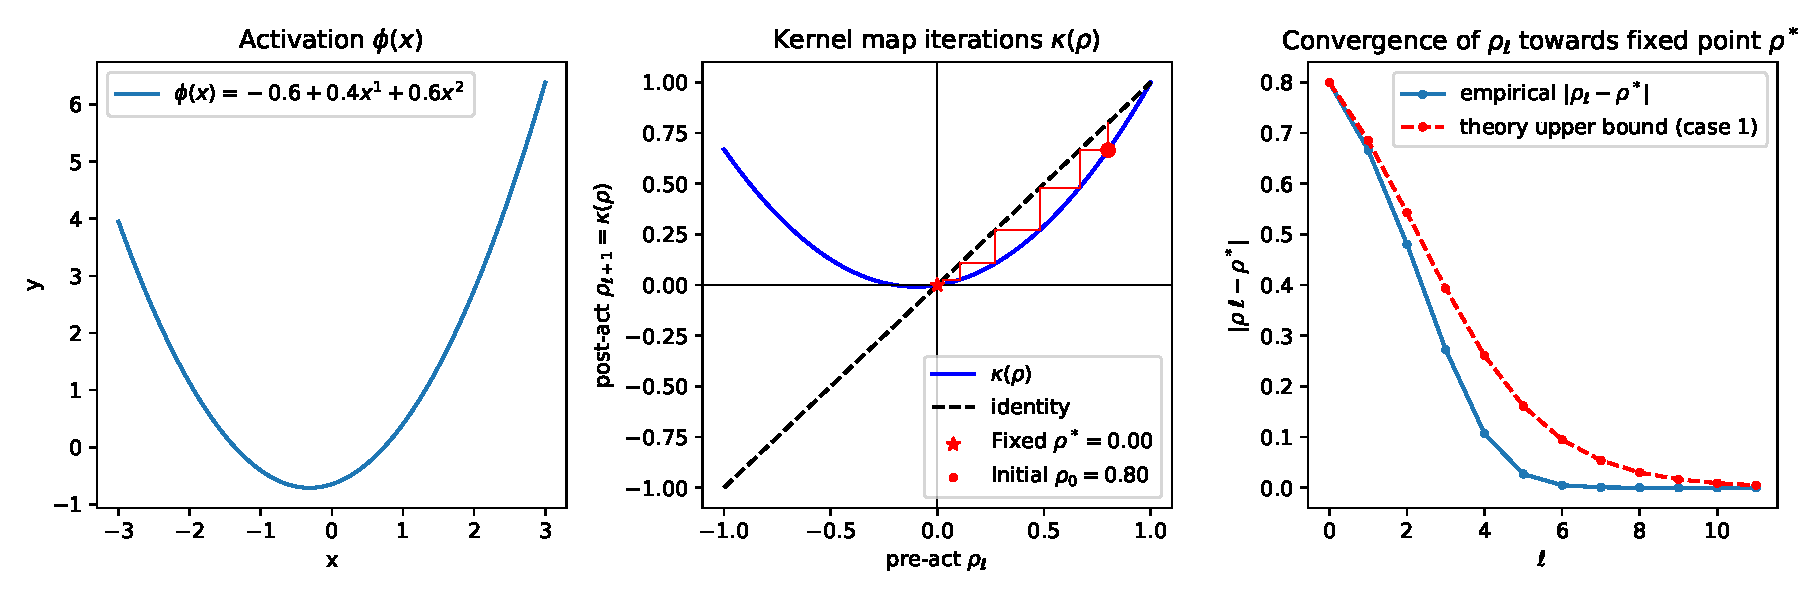
\includegraphics[width=\textwidth]{./kernel_map_convergence_case_0.pdf}
        \caption{\small Case 1}
    \end{subfigure}
    \hfill
    \begin{subfigure}[b]{0.7\textwidth}
        \centering
        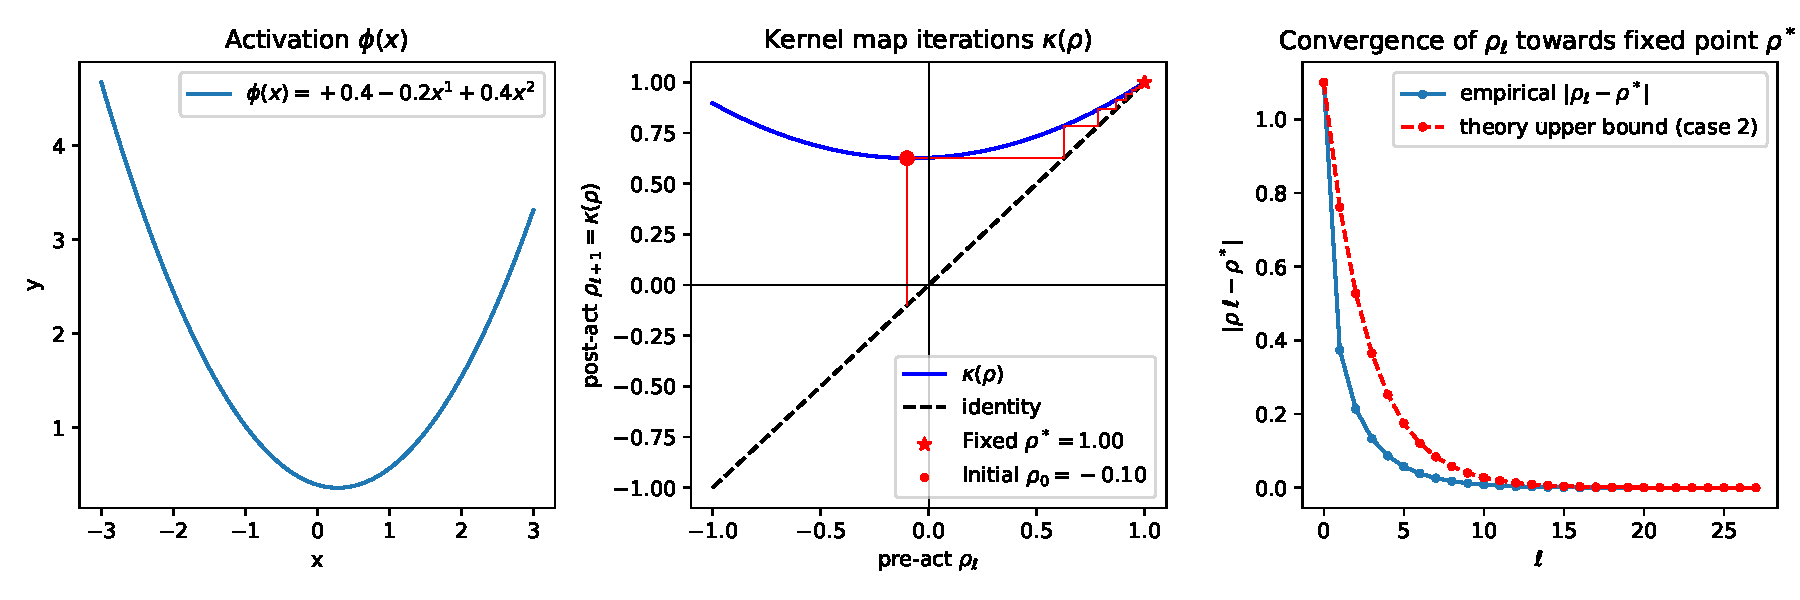
\includegraphics[width=\textwidth]{./kernel_map_convergence_case_1.pdf}
        \caption{\small Case 2}
    \end{subfigure}
    \\
    \begin{subfigure}[b]{0.7\textwidth}
        \centering
        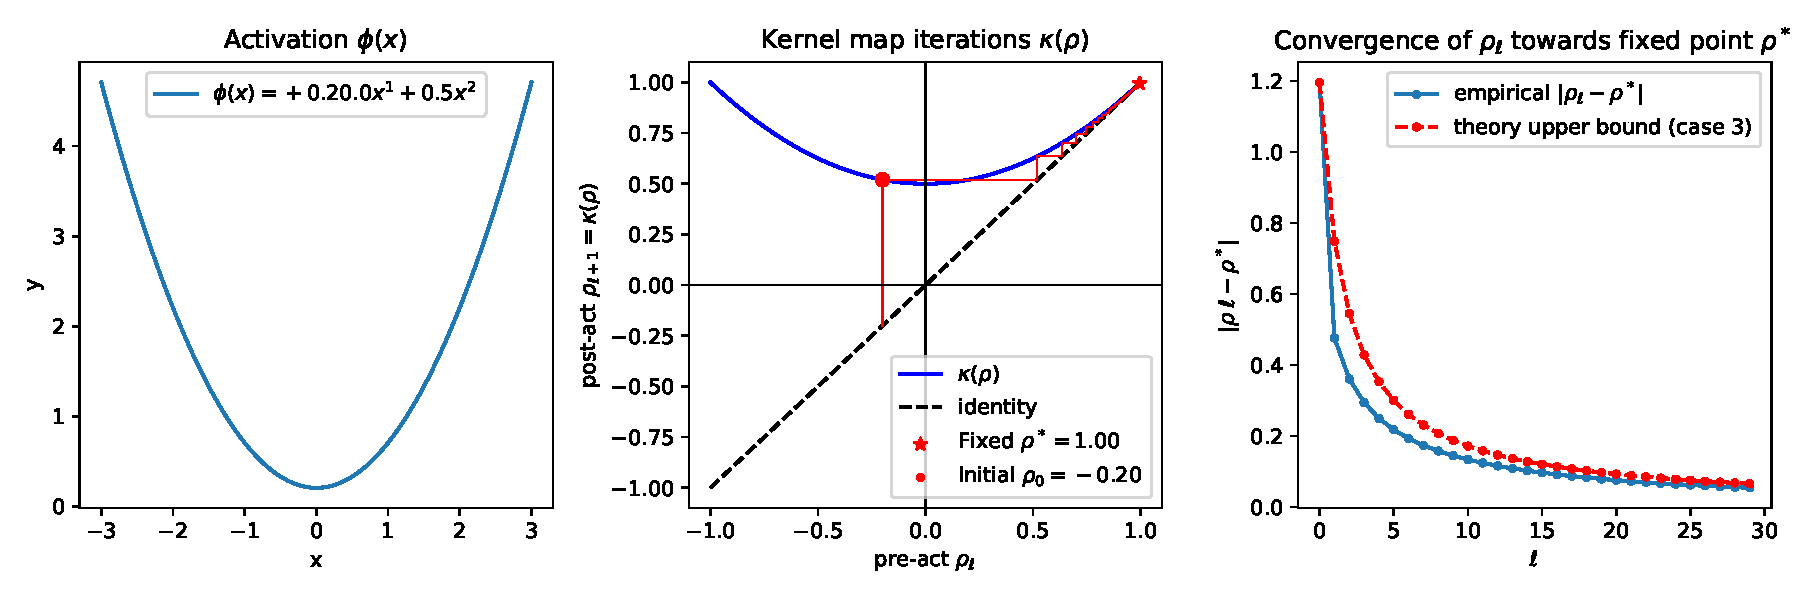
\includegraphics[width=\textwidth]{./kernel_map_convergence_case_2.pdf}
        \caption{\small Case 3}
    \end{subfigure}
    \hfill
    \begin{subfigure}[b]{0.7\textwidth}
        \centering
        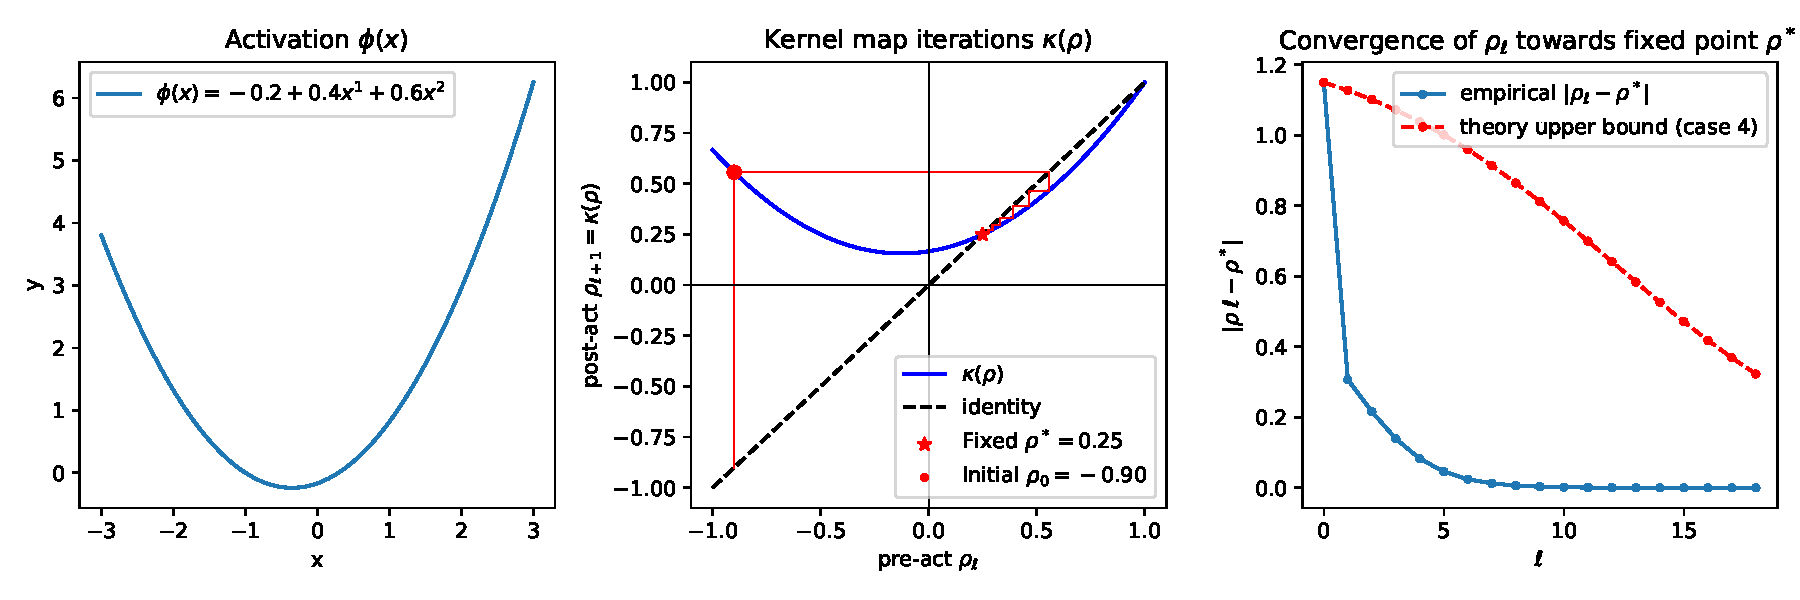
\includegraphics[width=\textwidth]{./kernel_map_convergence_case_3.pdf}
        \caption{\small Case 4}
    \end{subfigure}
    \caption{\small Validation of Theorem~\ref{thm:global_attract}, each corresponding to one of the four cases of the theorem. Left column shows the activation $\phi.$ The middle and right columns show the kernel map show fixed point iteration starting from $\rho_0,$ and applying $\rho_{\ell+1}=\kappa(\rho_\ell)$ for many steps. The middle column shows the kernel map, while the right column shows the distance to the fixed point $\rho^*$.}
    \label{fig:validation_plots}
\end{figure*}

\begin{figure*}[ht!]
    \centering
    \begin{subfigure}[b]{0.7\textwidth}
        \centering
        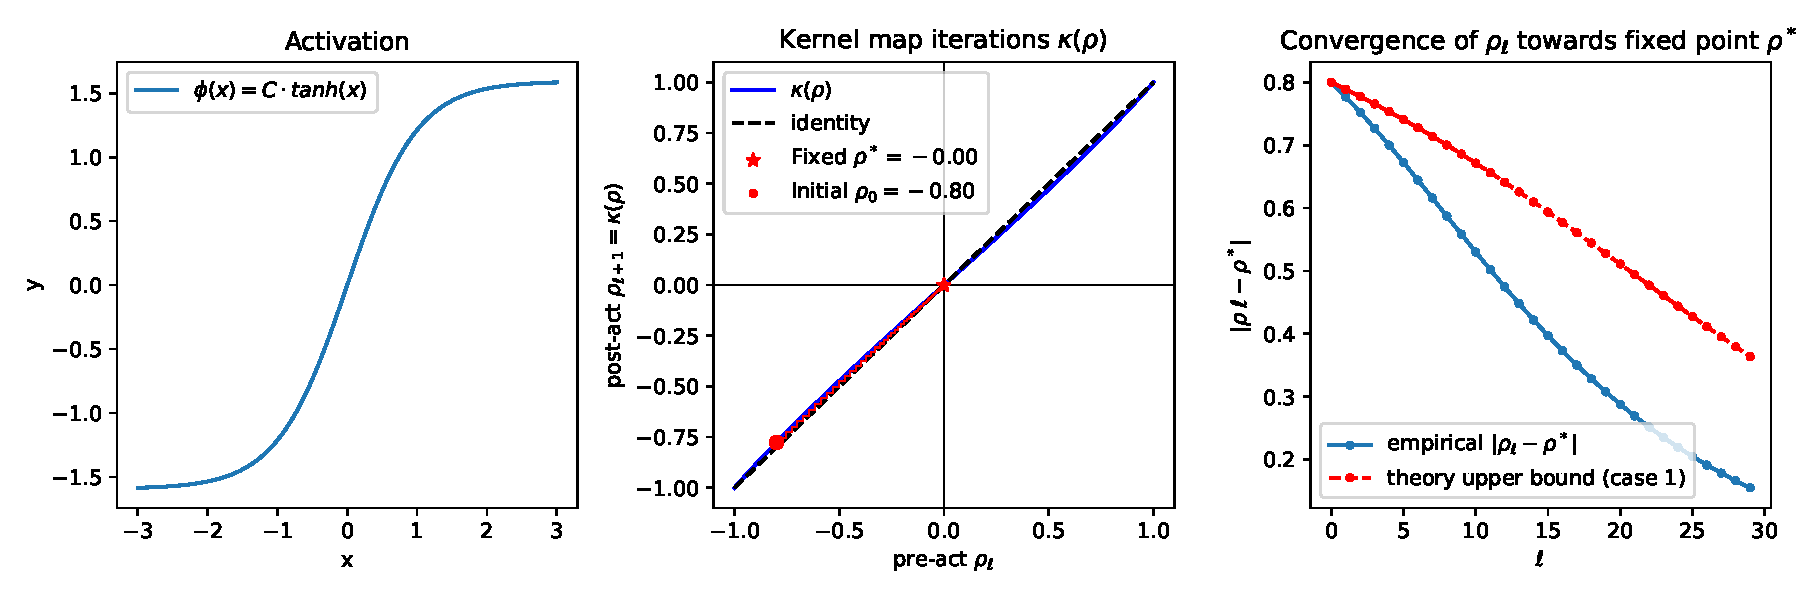
\includegraphics[width=\textwidth]{./kernel_map_convergence_case_0_tanh.pdf}
        \caption{\small Case 1. Tanh activation.}
    \end{subfigure}
    \hfill
    \begin{subfigure}[b]{0.7\textwidth}
        \centering
        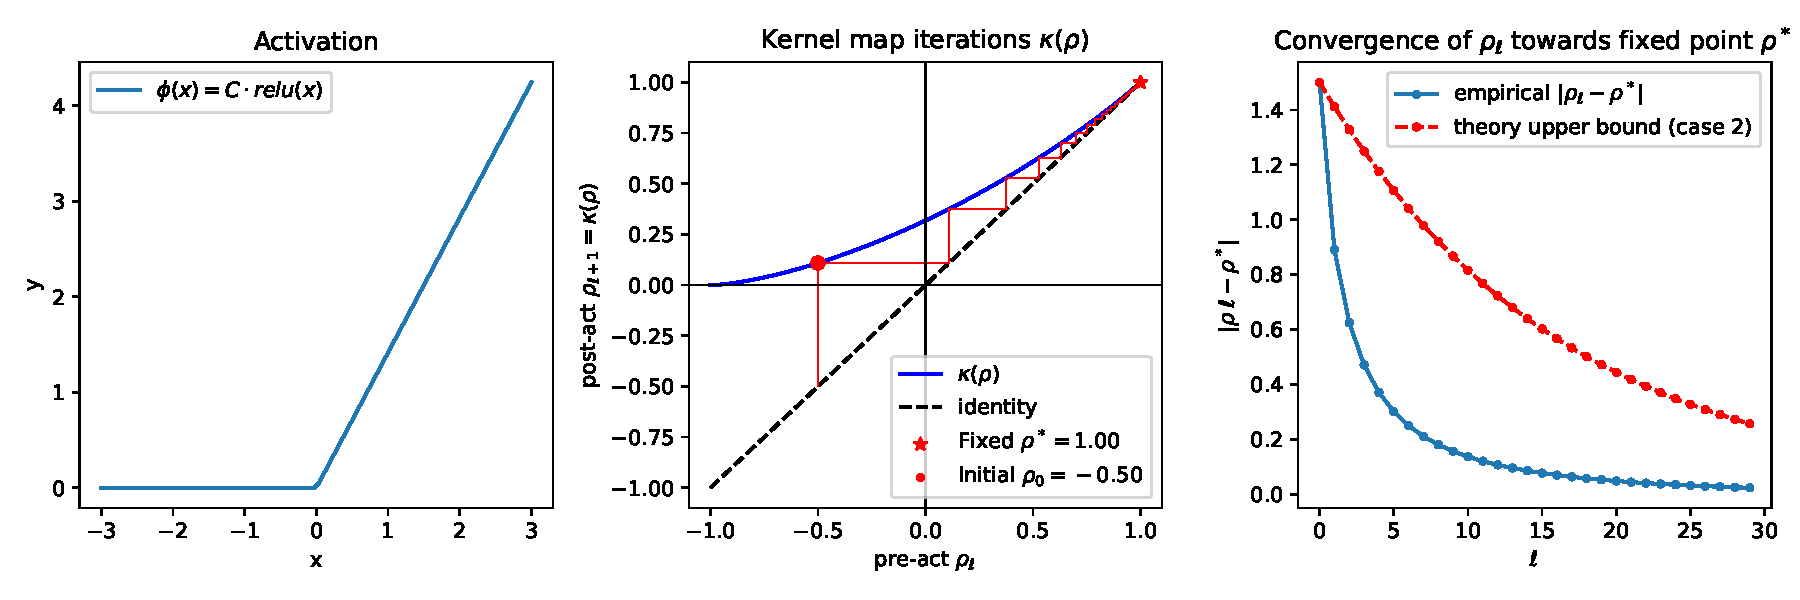
\includegraphics[width=\textwidth]{./kernel_map_convergence_case_1_relu.pdf}
        \caption{\small Case 2: ReLU activation.}
    \end{subfigure}
    \\
    \begin{subfigure}[b]{0.7\textwidth}
        \centering
        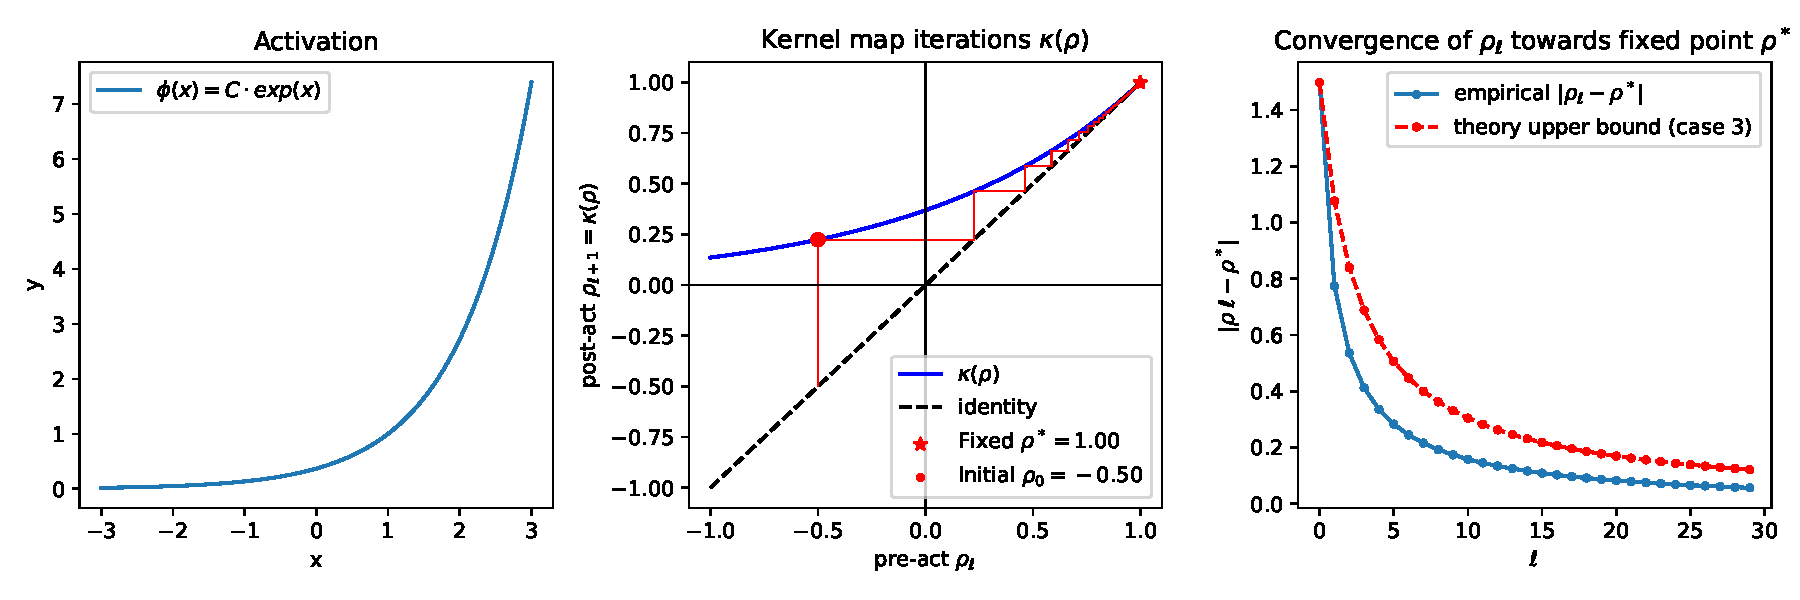
\includegraphics[width=\textwidth]{./kernel_map_convergence_case_2_exp.pdf}
        \caption{\small Case 3: Exponential activation.} 
    \end{subfigure}
    \hfill
    \begin{subfigure}[b]{0.7\textwidth}
        \centering
        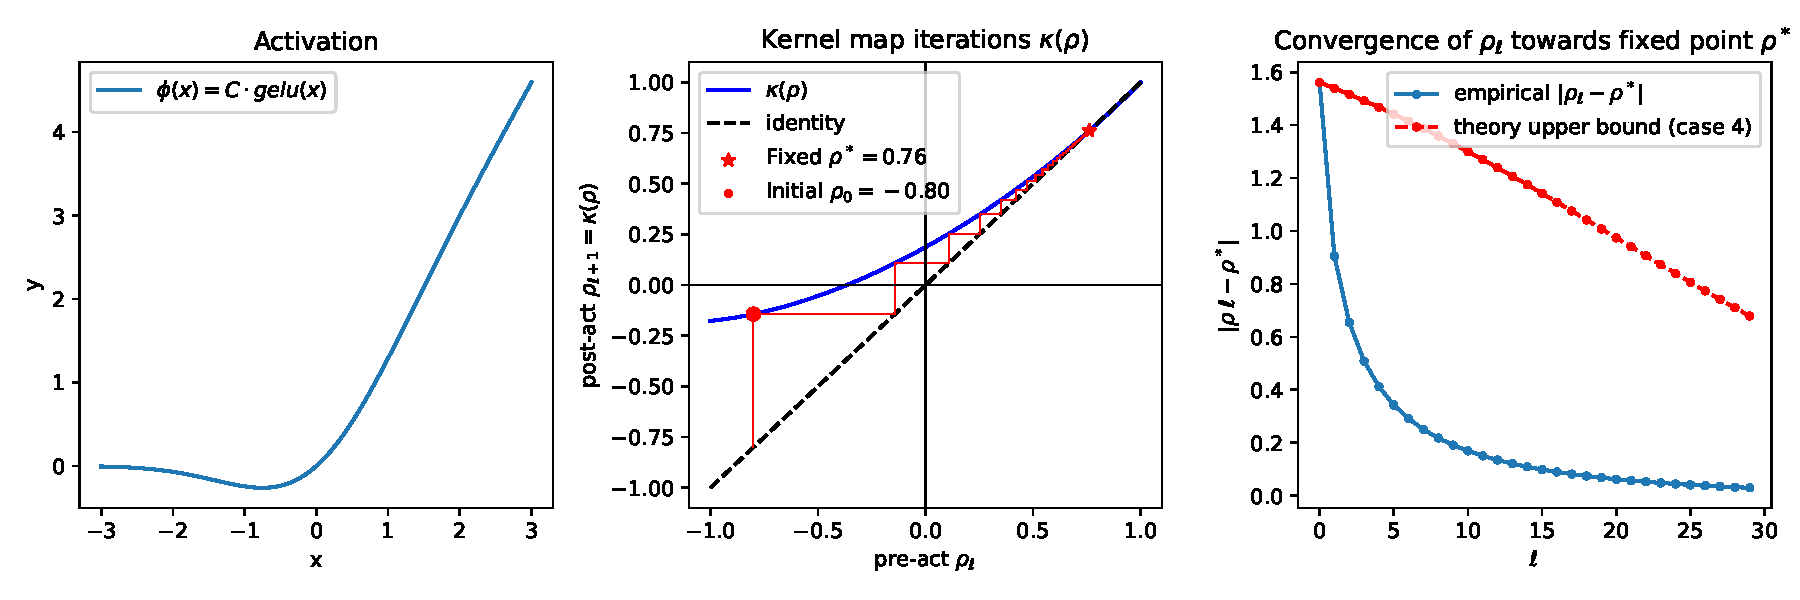
\includegraphics[width=\textwidth]{./kernel_map_convergence_case_3_gelu.pdf}
        \caption{\small Case 4: GELU activation.}
    \end{subfigure}
    \caption{\small Same as Figure~\ref{fig:validation_plots} for some commonly used activations. Note that because the raw activations do not necessariy obey $\E \phi^2(X)=1,$ we have to scale by some contant $C$ to make the activations obey the conditions of the theorem.}
    \label{fig:validation_plots_real_activations}
\end{figure*}

\section{Conclusion}

\bibliographystyle{apalike}
\bibliography{refs}

\end{document}
